%%%%%%%%%%%%%%%%%%%%%%%%%%%%%%%%%%%%%%%%%
% Masters/Doctoral Thesis 
% LaTeX Template
% Version 2.2 (21/11/15)
%
% This template has been downloaded from:
% http://www.LaTeXTemplates.com
%
% Version 2.x major modifications by:
% Vel (vel@latextemplates.com)
%
% This template is based on a template by:
% Steve Gunn (http://users.ecs.soton.ac.uk/srg/softwaretools/document/templates/)
% Sunil Patel (http://www.sunilpatel.co.uk/thesis-template/)
%
% Template license:
% CC BY-NC-SA 3.0 (http://creativecommons.org/licenses/by-nc-sa/3.0/)
%
%%%%%%%%%%%%%%%%%%%%%%%%%%%%%%%%%%%%%%%%%

%----------------------------------------------------------------------------------------
%	PACKAGES AND OTHER DOCUMENT CONFIGURATIONS
%----------------------------------------------------------------------------------------

\documentclass[
12pt, % The default document font size, options: 10pt, 11pt, 12pt
%oneside, % Two side (alternating margins) for binding by default, uncomment to switch to one side
english, % ngerman for German
onehalfspacing, % Single line spacing, alternatives: onehalfspacing or doublespacing
%draft, % Uncomment to enable draft mode (no pictures, no links, overfull hboxes indicated)
%nolistspacing, % If the document is onehalfspacing or doublespacing, uncomment this to set spacing in lists to single
%liststotoc, % Uncomment to add the list of figures/tables/etc to the table of contents
%toctotoc, % Uncomment to add the main table of contents to the table of contents
%parskip, % Uncomment to add space between paragraphs
%nohyperref, % Uncomment to not load the hyperref package
headsepline, % Uncomment to get a line under the header
]{MastersDoctoralThesis} % The class file specifying the document structure

\usepackage[utf8]{inputenc} % Required for inputting international characters
\usepackage[T1]{fontenc} % Output font encoding for international characters

\usepackage{lmodern} % Use the Palatino font by default

\usepackage[sorting=none,backend=biber,style=numeric,natbib=true]{biblatex} % User the bibtex backend with the authoryear citation style (which resembles APA)

\addbibresource{thesis.bib} % The filename of the bibliography

\usepackage[autostyle=true]{csquotes} % Required to generate language-dependent quotes in the bibliography

\usepackage{amssymb,amsmath,enumerate}
\usepackage{graphicx}                                                                                                                                 
\usepackage[font=small,hypcap]{caption}
\usepackage{subcaption}
\usepackage{algorithm}% http://ctan.org/pkg/algorithms
\usepackage{algpseudocode}% http://ctan.org/pkg/algorithmicx
\usepackage{pdflscape}
\usepackage{amsmath,amsthm}

\newtheorem{definition}{Definition}
\newtheorem{theorem}{Theorem}
%----------------------------------------------------------------------------------------
%	MARGIN SETTINGS
%----------------------------------------------------------------------------------------

\geometry{
	paper=a4paper, % Change to letterpaper for US letter
	inner=1.5cm, % Inner margin
	outer=2.8cm, % Outer margin
	bindingoffset=2cm, % Binding offset
	top=1.5cm, % Top margin
	bottom=1.5cm, % Bottom margin
	%showframe,% show how the type block is set on the page
}

%----------------------------------------------------------------------------------------
%	THESIS INFORMATION
%----------------------------------------------------------------------------------------

\thesistitle{A New Methodology For Combining Graph Kernels} % Your thesis title, this is used in the title and abstract, print it elsewhere with \ttitle
\supervisor{Prof. Alessandro \textsc{Sperduti}} % Your supervisor's name, this is used in the title page, print it elsewhere with \supname
\examiner{} % Your examiner's name, this is not currently used anywhere in the template, print it elsewhere with \examname
\degree{Laurea Magistrale} % Your degree name, this is used in the title page and abstract, print it elsewhere with \degreename
\author{Carlo Maria \textsc{Massimo}} % Your name, this is used in the title page and abstract, print it elsewhere with \authorname
\addresses{} % Your address, this is not currently used anywhere in the template, print it elsewhere with \addressname

\subject{Computer Science} % Your subject area, this is not currently used anywhere in the template, print it elsewhere with \subjectname
\keywords{} % Keywords for your thesis, this is not currently used anywhere in the template, print it elsewhere with \keywordnames
\university{Universit\`a degli Studi di Padova} % Your university's name and URL, this is used in the title page and abstract, print it elsewhere with \univname
\department{Dipartimento di Matematica} % Your department's name and URL, this is used in the title page and abstract, print it elsewhere with \deptname
\group{} % Your research group's name and URL, this is used in the title page, print it elsewhere with \groupname
\faculty{Facolt\`a di Informatica} % Your faculty's name and URL, this is used in the title page and abstract, print it elsewhere with \facname

\hypersetup{pdftitle=\ttitle} % Set the PDF's title to your title
\hypersetup{pdfauthor=\authorname} % Set the PDF's author to your name
\hypersetup{pdfkeywords=\keywordnames} % Set the PDF's keywords to your keywords

\begin{document}

\frontmatter % Use roman page numbering style (i, ii, iii, iv...) for the pre-content pages

\pagestyle{plain} % Default to the plain heading style until the thesis style is called for the body content

%----------------------------------------------------------------------------------------
%	TITLE PAGE
%----------------------------------------------------------------------------------------

\begin{titlepage}
\begin{center}

\textsc{\LARGE \univname}\\[1.5cm] % University name
\textsc{\large \deptname}\\[0.5cm] % Thesis type

 
\textsc{ Corso di Laurea Magistrale in Informatica}\\[0.5cm] % Thesis type
\textsc{\small Anno Accademico 2015-2016}\\[2.5cm] % Thesis type

\HRule \\[0.4cm] % Horizontal line
{\huge \bfseries \ttitle}\\[0.4cm] % Thesis title
\HRule \\[1.5cm] % Horizontal line
 
\begin{minipage}{0.4\textwidth}
\begin{flushleft} \large
\emph{Studente:}\\
\authorname\\1058513 % Author name - remove the \href bracket to remove the link
\end{flushleft}
\end{minipage}
\begin{minipage}{0.4\textwidth}
\begin{flushright} \large
\emph{Relatore:} \\
\supname % Supervisor name - remove the \href bracket to remove the link  
\end{flushright}
\end{minipage}\\[3cm]
 
%{\large \today}\\[4cm] % Date
%\includegraphics{Logo} % University/department logo - uncomment to place it
 
\vfill
\end{center}
\end{titlepage}

\cleardoublepage

%----------------------------------------------------------------------------------------
%	QUOTATION PAGE
%----------------------------------------------------------------------------------------

%\vspace*{0.2\textheight}
%
%\noindent\enquote{\itshape 'OMG this is so meta I cant even}\bigbreak
%
%\hfill clojure

%----------------------------------------------------------------------------------------
%	ABSTRACT PAGE
%----------------------------------------------------------------------------------------

\begin{abstract}
\addchaptertocentry{\abstractname} % Add the abstract to the table of contents

Graph mining and machine learning methods that use the graph representation have seen
a steady growth in success and proposed approaches during the last decades.
A number of improvements over the existing techniques, have recently been
proposed, further raising the performance limits.
These works typically address a specific weak point in a particular approach,
so a natural question one may want to answer is if a combination of these
improvements can outperform the single one.

To be able to efficiently and effectively answer to such questions, a tested way
of combining the various improvement is needed.
In this study we devise a general methodology to favor the implementation of these
combinations and test them in an easy and time-efficient way.

To warrant the generalization of the proposed methodology we analysed three
possible combination, namely we took three graph kernels that has recently
been extended with contextual information and combined the two versions for each
one.
The analyses are derived from a number of real world, publicly available
bio-chemical datasets.

Empirical results show that the proposed methodology is faster than current
state-of-the-art kernel machines while always maintaining comparable performances
and in some cases exceed those of the proposed baselines.
\end{abstract}

%----------------------------------------------------------------------------------------
%	ACKNOWLEDGEMENTS
%----------------------------------------------------------------------------------------

%\begin{acknowledgements}
%\addchaptertocentry{\acknowledgementname} % Add the acknowledgements to the table of contents
%
%I would deeply and sincerely like to thank\dots
%
%
%\end{acknowledgements}

%----------------------------------------------------------------------------------------
%	LIST OF CONTENTS/FIGURES/TABLES PAGES
%----------------------------------------------------------------------------------------

\tableofcontents % Prints the main table of contents

\listoffigures % Prints the list of figures

\listoftables % Prints the list of tables

\listofalgorithms

%----------------------------------------------------------------------------------------
%	ABBREVIATIONS
%----------------------------------------------------------------------------------------

%\begin{abbreviations}{ll} % Include a list of abbreviations (a table of two columns)
%
%\textbf{MKL} & \textbf{M}ultiple \textbf{K}ernel \textbf{L}earning\\
%\textbf{ODD} & \textbf{O}rdered \textbf{D}AG \textbf{D}ecomposition\\
%\textbf{ST} & \textbf{S}ub \textbf{T}ree\\
%\textbf{TCK} & \textbf{T}ree \textbf{C}ontext \textbf{K}ernel\\
%\textbf{ROC} & \textbf{R}eceiver \textbf{O}perator \textbf{C}urve\\
%\textbf{AUC} & \textbf{A}rea \textbf{U}nder \textbf{C}urve\\
%
%\end{abbreviations}

%----------------------------------------------------------------------------------------
%	PHYSICAL CONSTANTS/OTHER DEFINITIONS
%----------------------------------------------------------------------------------------

%\begin{constants}{lr@{${}={}$}l} % The list of physical constants is a three column table

% The \SI{}{} command is provided by the siunitx package, see its documentation for instructions on how to use it

%	Speed of Light & $c_{0}$ & \SI{2.99792458e8}{\meter\per\second} (exact)\\
%Constant Name & $Symbol$ & $Constant Value$ with units\\

%\end{constants}

%----------------------------------------------------------------------------------------
%	SYMBOLS
%----------------------------------------------------------------------------------------

%\begin{symbols}{lll} % Include a list of Symbols (a three column table)
%
%$\phi$ & features mapping function \\
%%Symbol & Name & Unit \\
%
%%\addlinespace % Gap to separate the Roman symbols from the Greek
%
%\end{symbols}

%----------------------------------------------------------------------------------------
%	DEDICATION
%----------------------------------------------------------------------------------------

%\dedicatory{To my parents, to whom I owe this achievement.}
%{To my friends that, even though a great distance is between us most of the time,
%managed to be of invaluable help and motivation.} 
%{To you, that made me believe in my dreams again.}

%----------------------------------------------------------------------------------------
%	THESIS CONTENT - CHAPTERS
%----------------------------------------------------------------------------------------

\mainmatter % Begin numeric (1,2,3...) page numbering

\pagestyle{thesis} % Return the page headers back to the "thesis" style

% Include the chapters of the thesis as separate files from the Chapters folder
% Uncomment the lines as you write the chapters

% Chapter 1

\chapter{Introduction} % Main chapter title
\label{Chapter1} % For referencing the chapter elsewhere, use \ref{Chapter1} 

This chapter presents a brief overview of the present thesis.
First we introduce some basic concept about data and knowledge along with some examples,
then the main contribution is explained with some more in-depth discussion,
followed by the document outline.

\section{Relationship between data and knowledge}

The current amount of digital data produced daily is estimated to be in the realm of 
ZettaBytes ($1~ZB = 10^{12}~GB$) \cite{idc}.
Of this amount, only a small fraction sees actual processing and interpretation,
mainly because while the flow of information is steady, the available resources
devoted to the task are often limited \cite{idc}.
Moreover in some cases the rapidity at which a meaningful interpretation of the 
raw data has to be produced is critical.
Hence, just the plain fact of owning the data does not imply that some useful 
information pattern can be derived from it; in fact the whole discipline of \emph{Data Mining}
was born with the intent of derive \emph{knowledge} that ``we don't know we don't know''.

Most of data mining techniques draw from a variety of other fields like Statistics,
Computer Science, Information Theory and Mathematics just to mention a few.
This discipline rests its theoretical foundation upon the field of \emph{Machine Learning},
the discipline that studies algorithms and techniques that allow a machine
to learn a concept (or an approximation of it) from a set of examples.
These algorithms start from limited evidence and try to build up a general model
by refining an initial \emph{hypothesis}.
Machine Learning is mostly useful when either an exact solution to the considered
problem is computationally infeasible or the problem specification
is rather vague or not unambiguously defined, leaving to the algorithm the burden
of exploration.

One of the pivotal concepts of this field is data \emph{representation}.
For the most part, data is collected and stored in unstructured form, i.e. vectors,
and a lot of machine learning techniques are tailored to this representation.
In the last decades some approaches tried to address those problems whose data cannot
be represented in vectorial form or whose representation in this form would cause
information loss.
%----------------------------------------------------------------------------------------

\section{Why structured data}
\label{sec:why}
% ci sono un sacco di dati strutturati
% c'e` la necessita` di applicare machine learning
% se li rappresentiamo come vettori non va bene perche` si perde struttura e piu`
% cresce il mapping piu` trattarlo diventa difficile.

The increasing amount of available structured data has made it necessary to develop
machine learning methods that can effectively deal with it.
More specifically some work has been done to devise methods that could learn
directly from graphs, a very useful kind of \emph{structured data} that sees many
important real-world applications nowadays, encompassing the fields of Computational
Biology, Computer Vision and Natural Language Processing.
For these applications it is natural to collect data that carries an inherent
amount of information concerning its structure.
That is, some data is naturally structured, e.g. molecular graphs or a sentence parse tree,
and representing it in vectorial form would inevitably cause a loss of information about
its structure.
There are some known ways of adding structural information to a vectorial representation,
with the addition of meta-data for instance, but this approach can render the
whole representation more cumbersome and potentially too complex to be treated
efficiently.

Graphs are a structured data form that can represent a great deal of different
information depending on the domain of application.
Graphs have multiple levels of information semantics and each level can have
different connotations, e.g. consider the set of edges, they can represent
different notions of link between two nodes while maintaining the same
representation.
Beside edges, that express a kind of local ``relationship''
information among the nodes, we have information stored at the node level in the
labels, where some qualitative or quantitative data may be present.
At a higher level we have topological information, which can be
viewed like an extended relationship level, and finally the information that can
be derived by looking at the shape of the graph such as notions
of connectivity, density etc.

\subsubsection{Examples}
\label{subsubsec:examples}

Chemical compounds are naturally represented by their molecular graph that carries
a lot of information about the structure of the molecule such as which atoms are
bound together; a simple graph representation of a molecule is given in Figure \ref{fig:chem}.
Most of the benchmark datasets employed in this study contain chemical compounds
represented in a similar way.

\begin{figure}[ht]
    \centering
    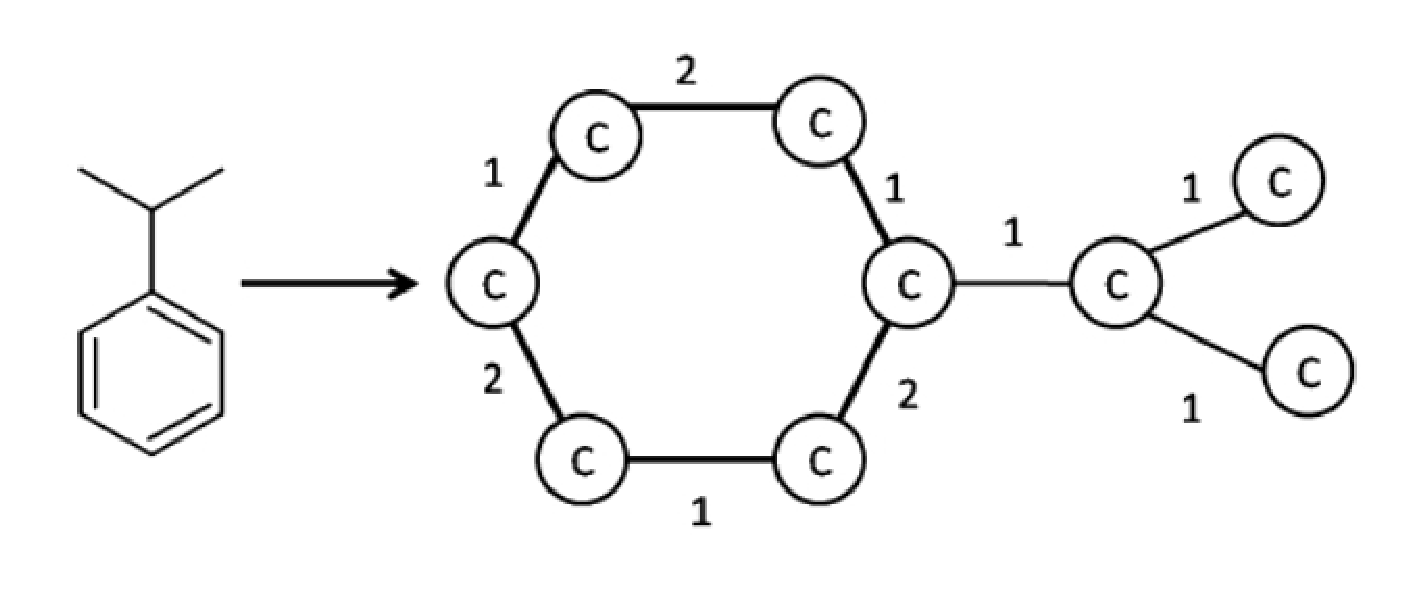
\includegraphics[scale=0.4]{Figures/chcomp}
    \caption{A molecule representation for a chemical compound and its representation
    as a graph; the nodes represent the atoms, the edges represent the chemical bounds and
    are labeled accordingly.}
    \label{fig:chem}
\end{figure}

Graph structured data has proven useful in the classification of non-coding RNA
molecules, modeled as shown in Figure \ref{fig:bio} \cite{nnavarin, conf/psb/KarklinMH05},

\begin{figure}[ht]
    \centering
    \begin{subfigure}{.4\textwidth}
        \centering
        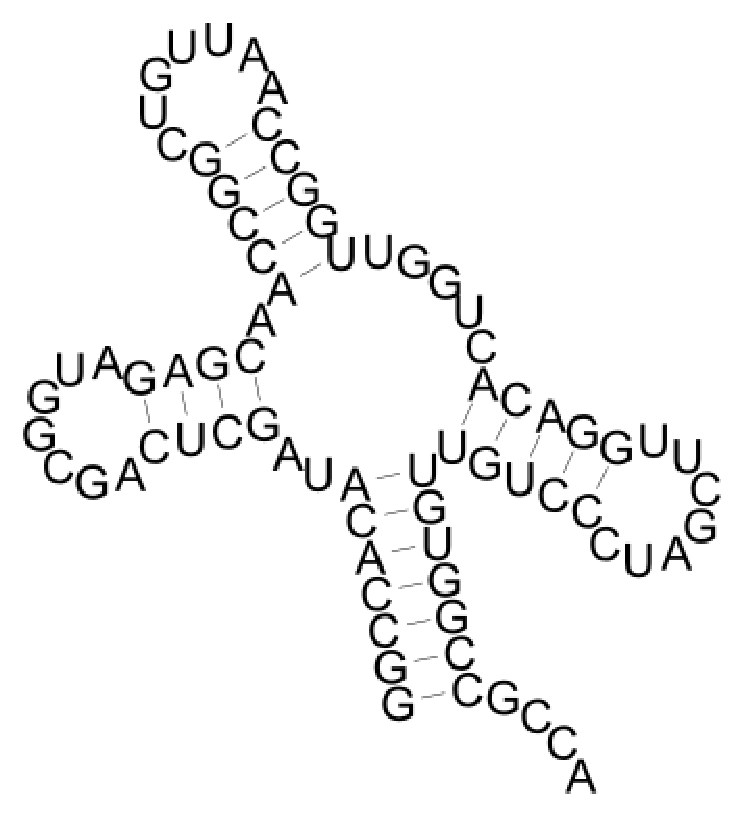
\includegraphics[width=\linewidth]{Figures/rna}
        \label{fig:rna}
        \caption{}
    \end{subfigure}
    \begin{subfigure}{.4\textwidth}
        \centering
        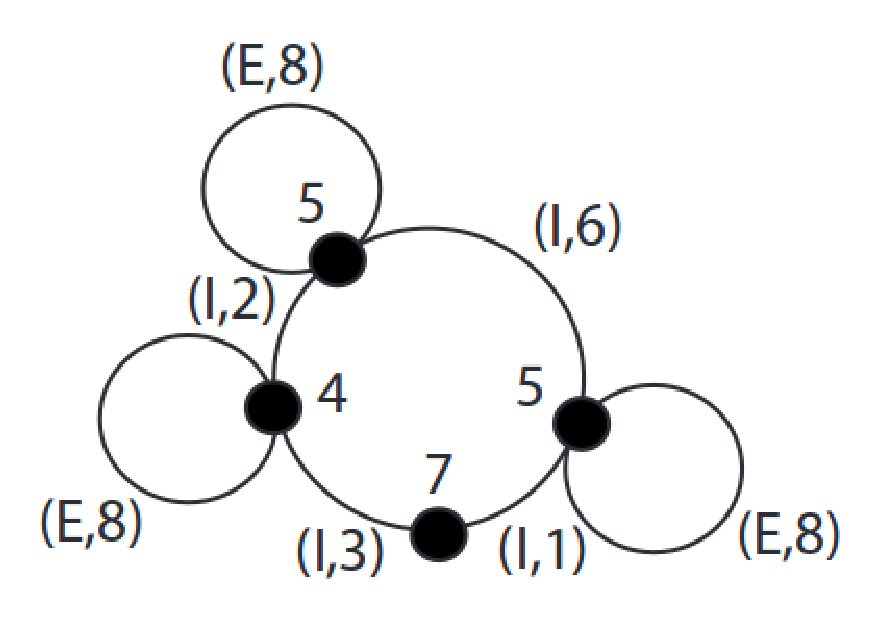
\includegraphics[width=\linewidth]{Figures/ldgrna}
        \label{fig:ldg}
        \caption{}
    \end{subfigure}
    \caption{a) RNA molecule graph representation and b) the same molecule represented
        as a labeled dual graph \cite{conf/psb/KarklinMH05}.}
    \label{fig:bio}
\end{figure}

Natural Language Processing is another field where graph representation is often used
as the basis for elaborate meaning extraction, as is the case for building opinion
lexicon from users review \cite{10.1371/journal.pone.0079294}, see Figure \ref{fig:wordrel}.

\begin{figure}[ht]
    \centering
    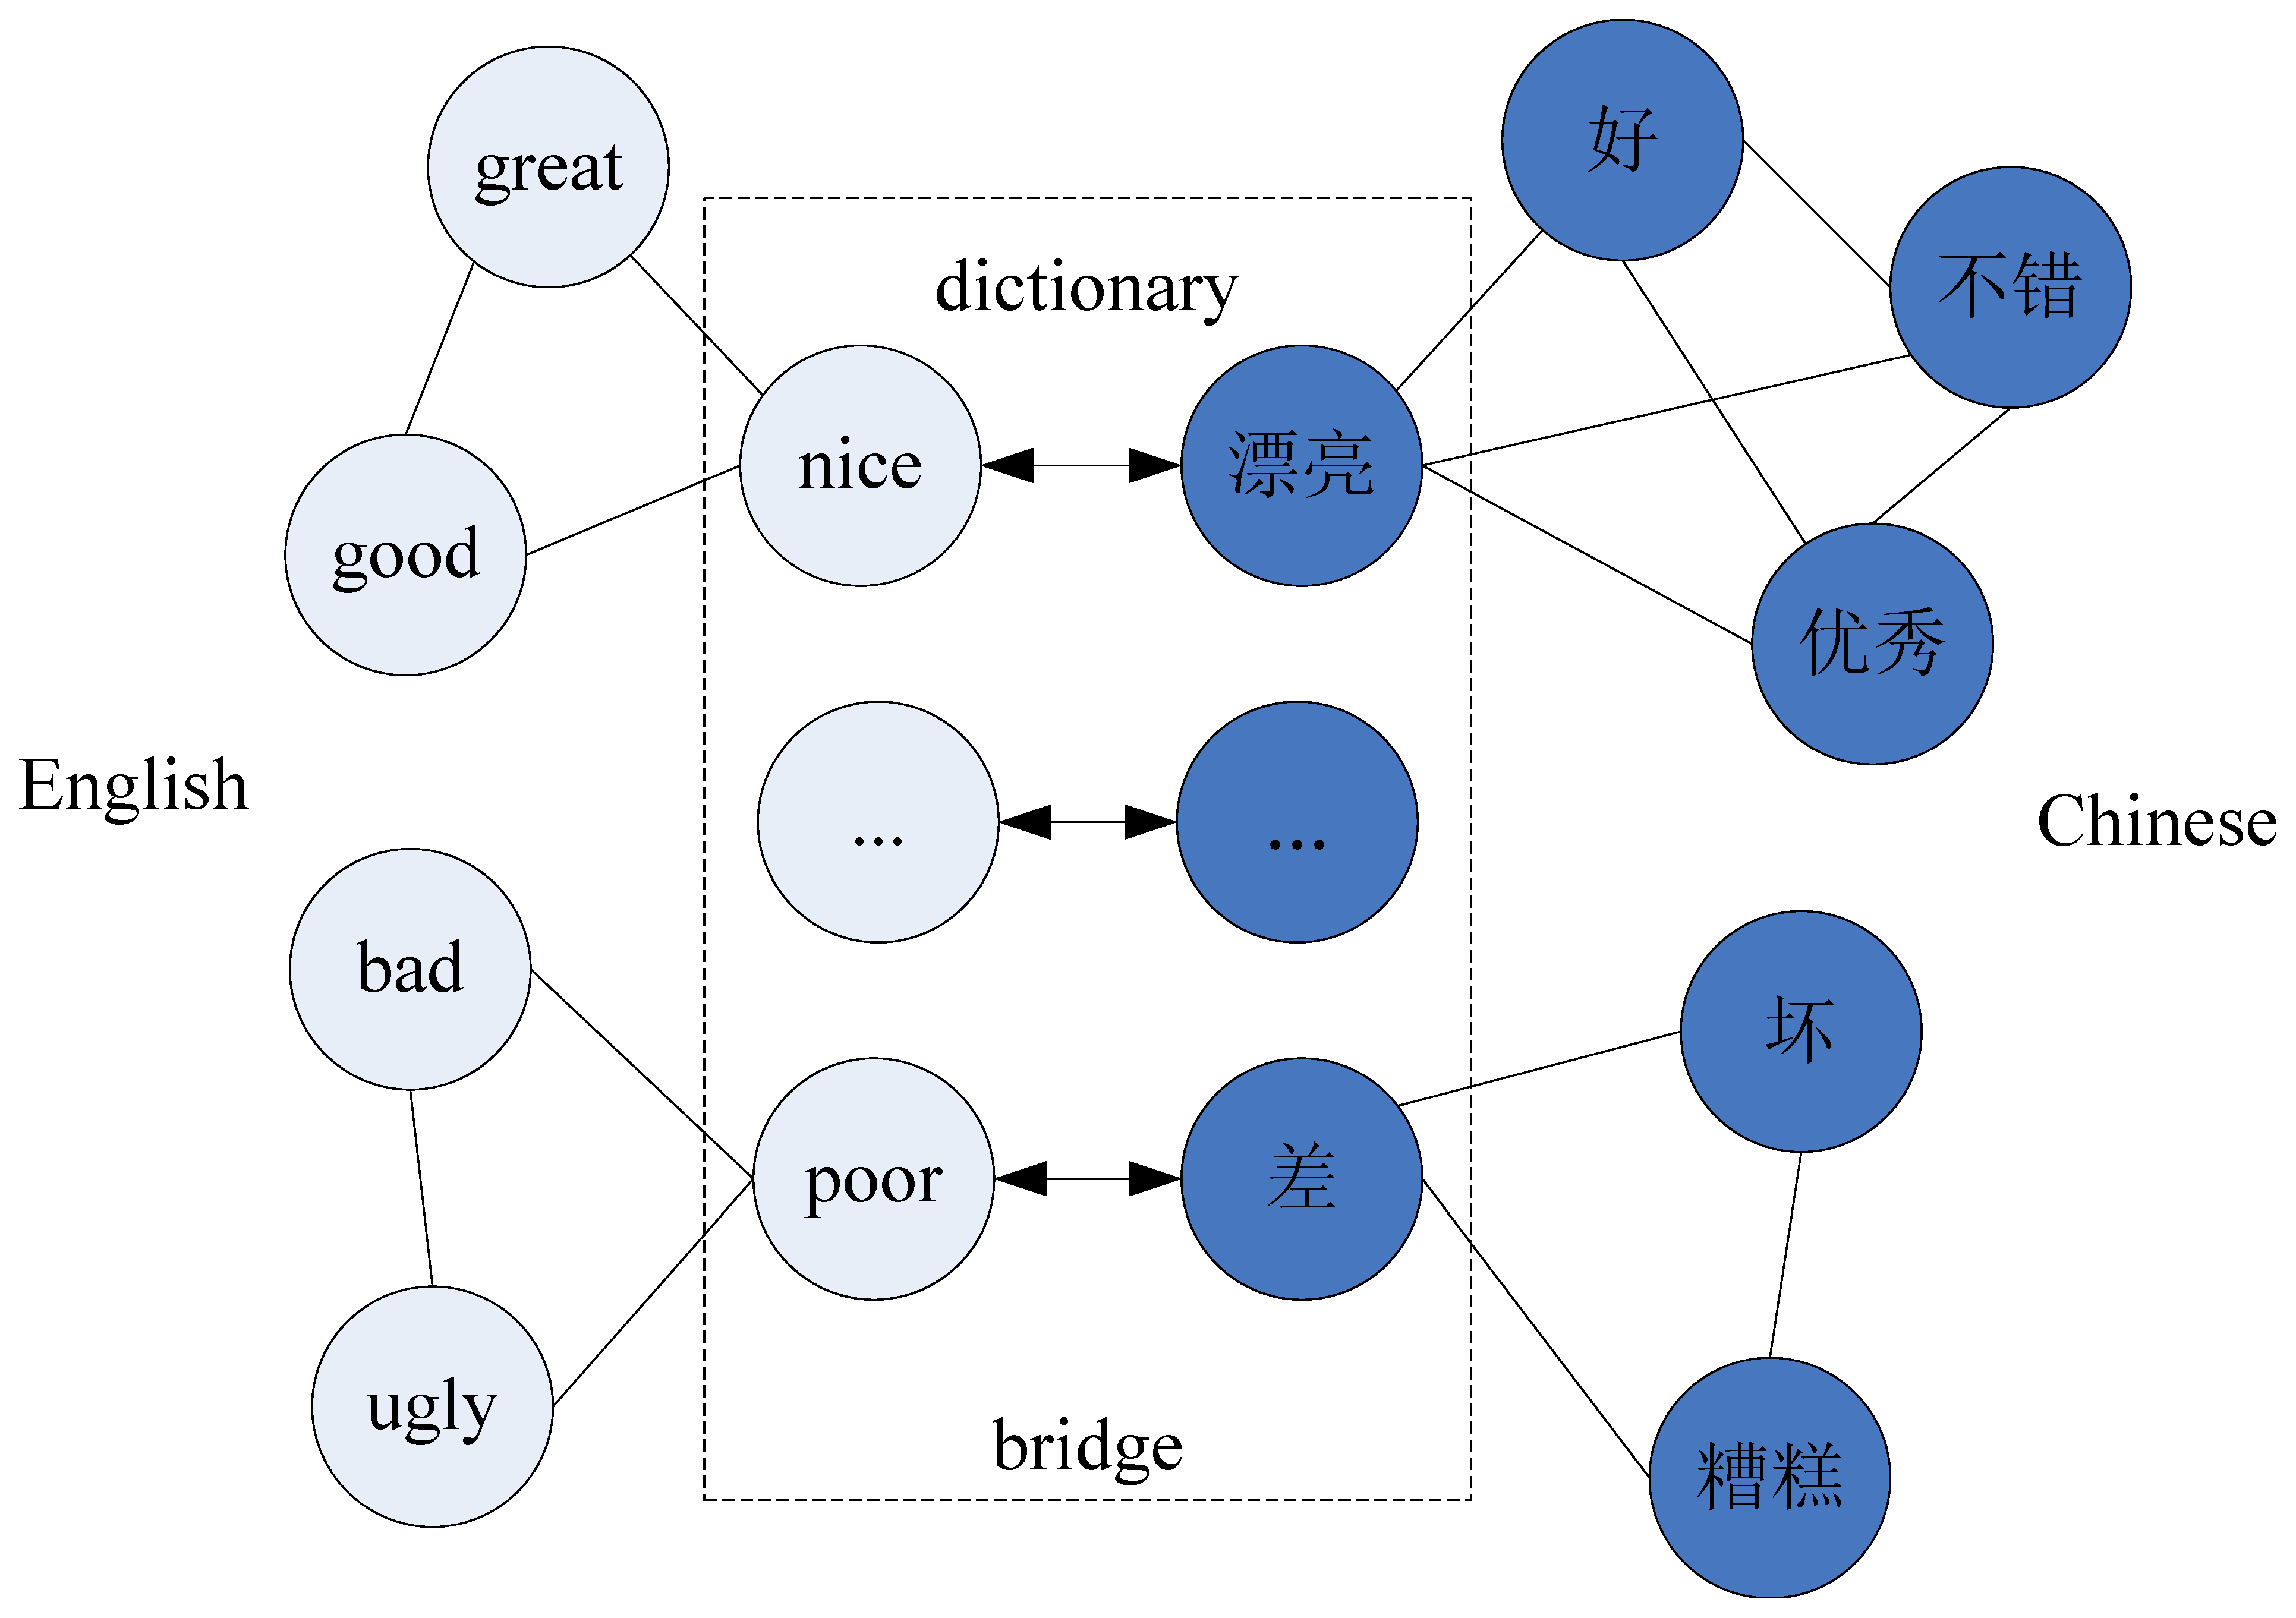
\includegraphics[width=.6\linewidth]{Figures/wordrel}
    \caption{Example of graph representation of words relationships in a multilingual
    context \cite{10.1371/journal.pone.0079294}.}
    \label{fig:wordrel}
\end{figure}

In Computer Vision a prominent application that uses graph representation is
the so-called scene understanding or scene modelling task, i.e. a scene is divided
into semantically meaningful areas which can be seen as nodes of a graph whose
edges are the adjacency relations between the areas \cite{journals/corr/abs-1108-4079},
an exemplification of this is given in Figure \ref{fig:scene}.

\begin{figure}[ht]
    \begin{subfigure}{.45\linewidth}
        \centering
        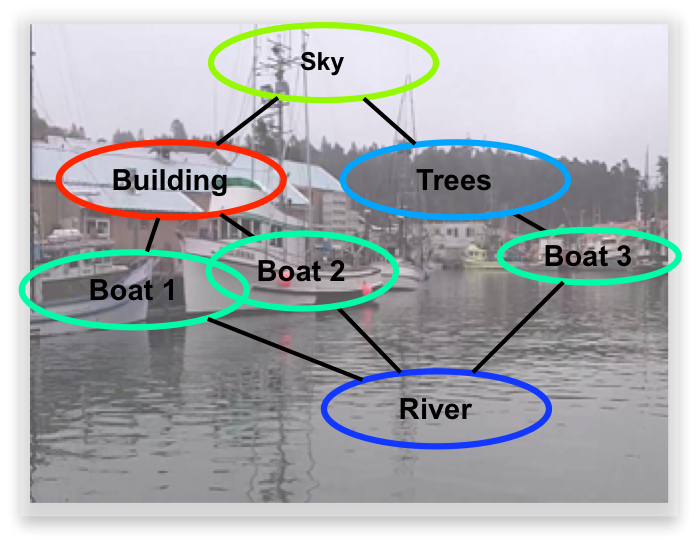
\includegraphics[width=\linewidth]{Figures/scene}
        \caption{}
        \label{fig:scene}
    \end{subfigure}
    \begin{subfigure}{.45\linewidth}
        \centering
        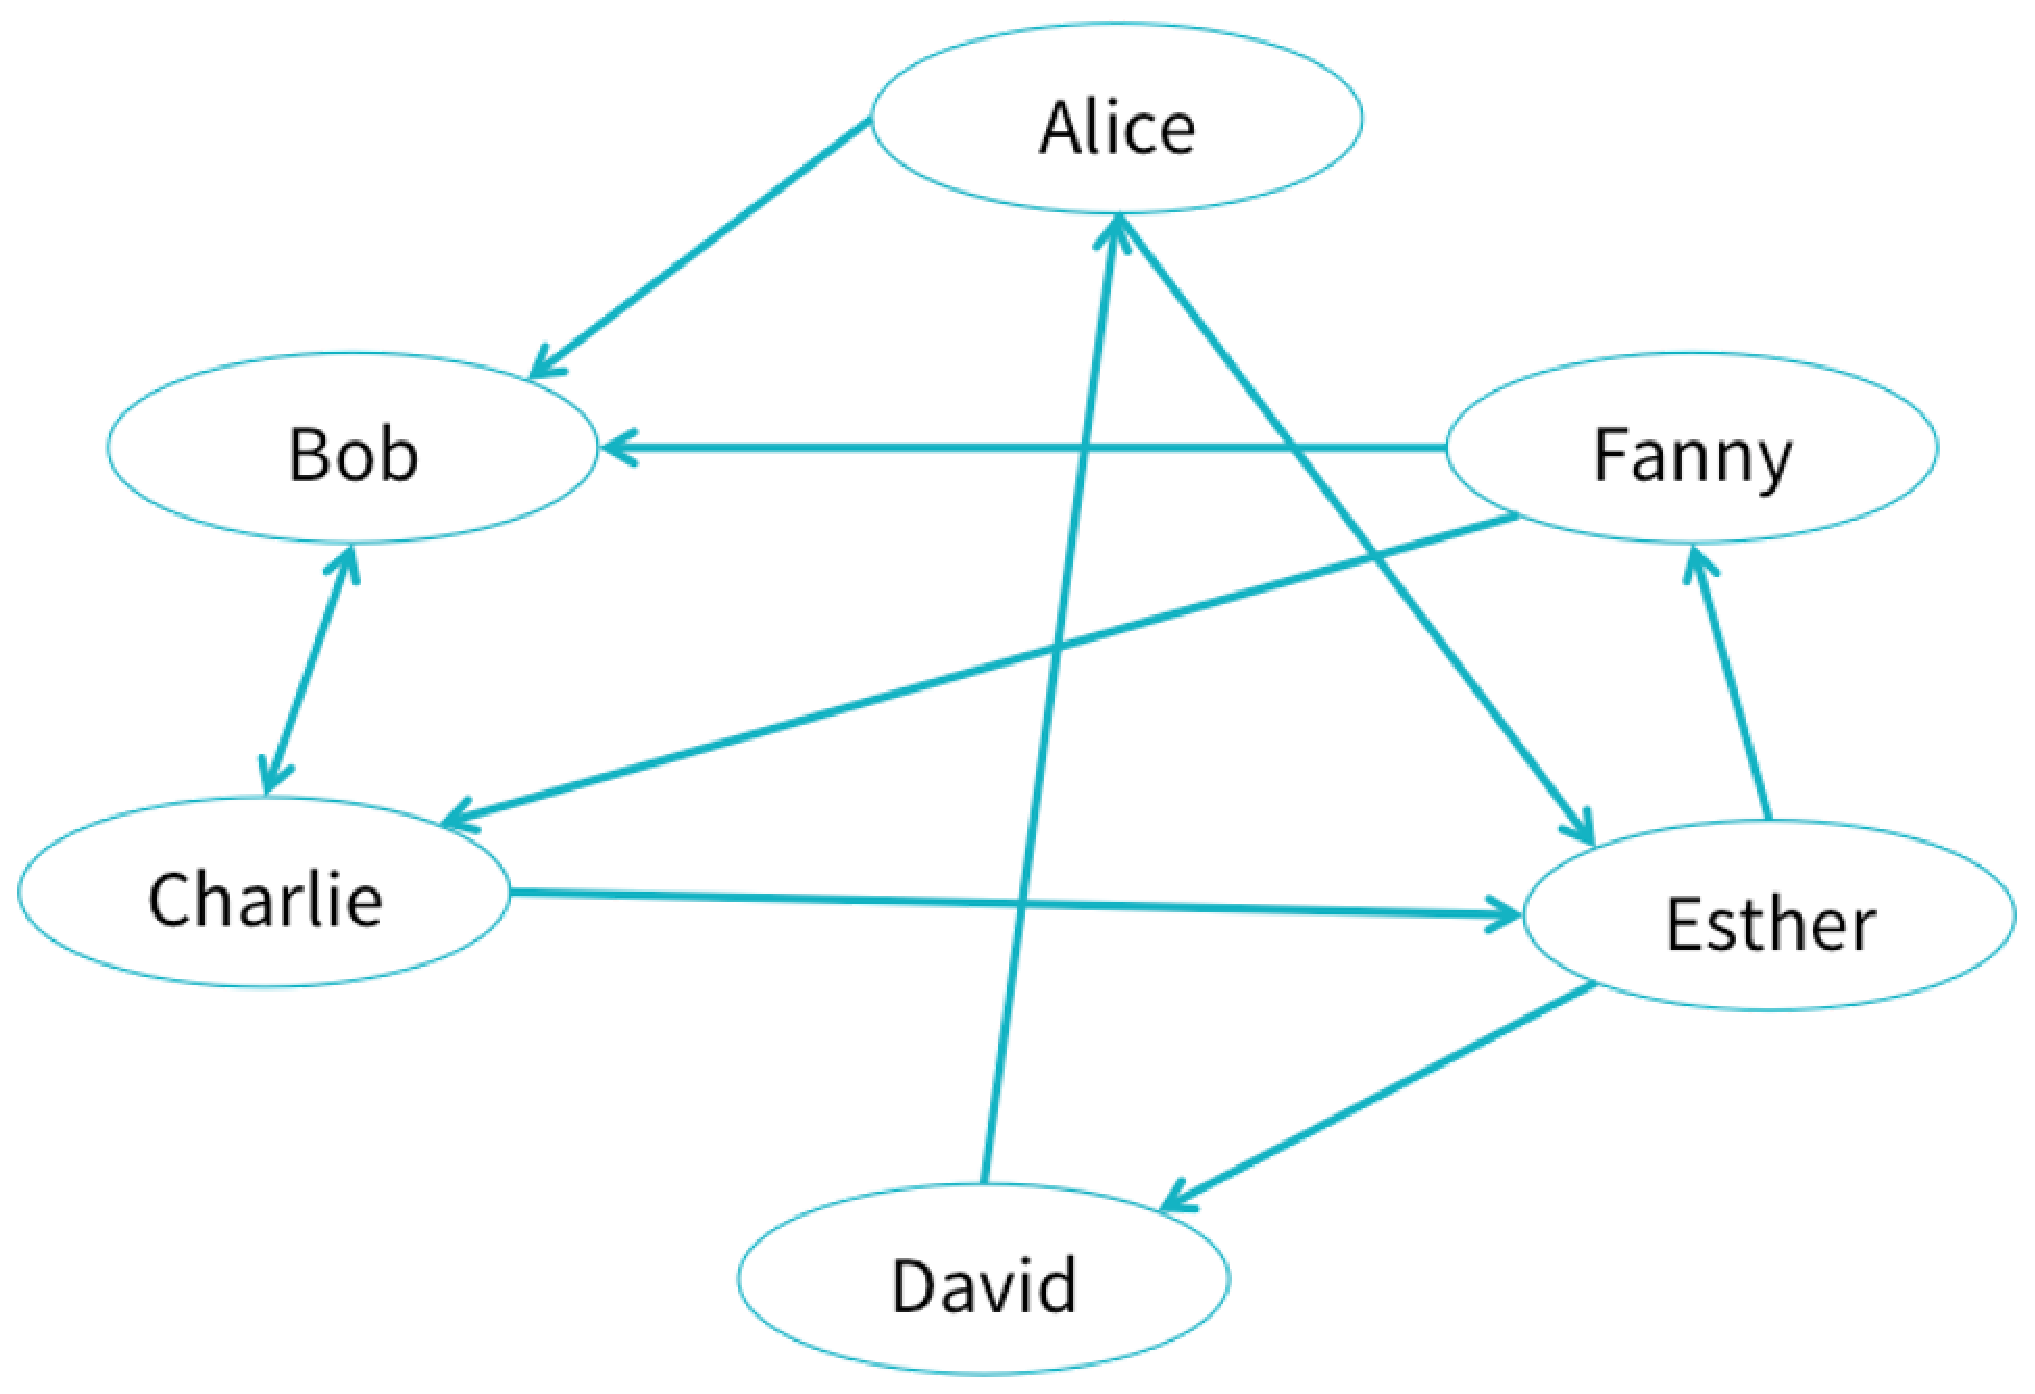
\includegraphics[width=\linewidth]{Figures/socialnetwork}
        \caption{}
        \label{fig:network}
    \end{subfigure}
\caption{a) Scene understanding via graph decomposition in Computer Vision. b)
        An example of a social graph where the nodes represent people and 
        the edges the property of ``knowing someone''.}
\end{figure}

Finally, graphs deriving from the inherently structured organization of every social
network can lead to a large number of mining possibilities given the vast
amount of data available \cite{gundecha2012mining}.
Figure \ref{fig:network} shows an example of a graph representing social relationships.
%----------------------------------------------------------------------------------------

\section{Graph kernel learning}

Given the wealth of available data, how can we learn from graphs? A first \emph{structure-based}
approach consists in designing an \emph{ad-hoc} vectorial representation for the
particular kind of graphs being considered.
A major downside of this approach is that a renewed effort for the 
design of a new representation is needed every time a new type of data
is encountered.

Another way to address the problem of graph learning is to adapt the existing methods
to work directly on graphs, thus allowing the exploitation of the existing techniques.
Some recently proposed works \cite{DBLP:conf/sdm/MartinoNS12, NIPS2009_3813}
embed graph specific knowledge into well established \emph{kernel methods}
that, given the inherent decoupling between the data representation and the learning
algorithm that they provide (more on Section \ref{subsec:introkm}), represent a
more general approach.

This thesis focuses on these kernel methods, and their use on a binary classification
task in a supervised setting that is, a task in which the machine learning algorithm
has to separate (classify) two sets of already labelled samples (hence ``supervised'').
In the following sections we assume to be operating in this scenario.

\subsection{Kernel methods}
\label{subsec:introkm}

Kernel methods are a collection of techniques that rely on an implicit representation
of the data and a well defined measure of similarity between samples to perform
the learning task.
These methods have two main components: a domain specific function to compute the
samples similarity score, called \emph{kernel function}, and a general purpose
learning algorithm, often called \emph{kernel machine}, to combine the information provided by the
kernel function in order to separate the samples.

Kernel functions implicitly map examples in a high dimensional space, commonly
referred to as \emph{feature space}, and define the similarity score as a dot
product in this space.
Specific domain knowledge gets embedded in the learning process through the definition
of the kernel function that becomes the only interface between the data
and the learning algorithm.
The explicit representation of the feature space is never accessed by the algorithm
that refers to it only implicitly through the kernel function.
This is commonly known as the \emph{kernel trick} and the reason behind it is 
that computing the dot product for each pair of samples in a high dimensional space
would be infeasible, but can be avoided thanks to the generally more efficient
kernel function since they are equivalent (Section \ref{subsec:kernelfunc}).

Kernel machines are learning algorithms that employ the similarity measures defined
by kernel functions to find a linear separator in a high dimensional feature space
since it is usually easier; once a separator has been found, it is mapped back
to the original input space from where the data was generated.
One of the most adopted methods is the Support Vector Machine (SVM) \cite{Cortes&Vapnik:1995}
which is a binary classifier that tries to find a separator that maximizes the \emph{margin}
between two sets of labelled samples that is, the distance between the separator and the
nearest sample of each class.
SVMs employ the samples pairwise distance as their similarity measure.

\subsection{Hyper-parameter selection}
\label{subsec:hyper1}

Most learning methods have parameters that need tuning, i.e. in order to achieve
good generalization performances each value has to be selected from a set of
possible choices according to a performance measure.
These parameters, often referred to as \emph{hyper-parameters}, define a
\emph{parameter space} characterized by their number, and by the size and type
of their domains.
This space can be potentially infinite and it is usually highly non-convex, making
the search for a global optimum very hard, if any exists.

For this reason the selection procedure often involves a limited search on the parameter space
that is, a set of values for each parameter is fixed, possibly after a discretization,
and all the combinations are tested to find the best one.
However, in order to be useful the sampling on the parameter space needs to be adequate:
even with a heuristic approach the complexity of this search can still be daunting because
it depends on the number of parameters.

In the context of kernel learning hyper-parameters can be found on two levels:
parameters relative to the kernel function and parameters that belongs to the
kernel machine (solver).
The parameters of the former typically influence the feature space being generated,
directly affecting the expressiveness of the similarity measure, i.e. the ability
to discern between two different samples.
The parameters of the solver are usually employed as regularization factors,
as is the case for the SVM, where its only hyper-parameter is used to balance the trade-off between a good
(generalizing) separator and empirical error.
Once the solver has been chosen, the parameter space is determined by the kernel
hyper-parameters hence, the kernel choice can greatly affect the computational
performances of the whole approach.
Moreover, often the kernel has to be selected in a similar way, thus increasing the
computational burden even more.

\subsection{Validation procedures}
The learning process is composed of two main phases, the training phase and
the test phase.
Briefly, in the training phase a model is built trying to approximate a concept, its performances
are then assessed during the test phase.
Each phase employs a different set of data, training data and test data respectively,
that is sampled from the original dataset.
Hyper-parameter values can deeply affect these two phases, in particular
because they determine which hypotheses are selected by the learning algorithm.
There are two main phenomena that are influenced by the values selected for the
hyper-parameters.

On one hand we have \emph{overfitting}, which happens when the hypothesis
(model) returned by the training phase is able to correctly classify the training data
but performs poorly on new instances that get presented to it, i.e. the test data.
This can happen because the selected hyper-parameter values render the model so
complex that it fits to spurious properties of the training data.

On the other hand we have \emph{underfitting} which consists in the hypothesis skewing
in a direction that makes it unable to grasp the full complexity of the data resulting
in a high classification error even on the training data.
This can be due to the model being too simple because of the chosen parameter values. 

In general we want to avoid the occurrence of either of these two phenomena:
typically a way to do this is to perform hyper-parameter selection employing
a \emph{validation set}, that is a fixed subset of the data left out from the
training phase and used to validate the performances of a model built according
to a given set of values for the parameters.
In this case the validation set coincides with the test data.
To reduce the bias, i.e. the distortion deriving from the fixed selection of
the validation set, a k-fold cross-validation technique is employed: the
data is split into $k$ subsets, $k-1$ become the training set while the last one
is used as the validation set; this procedure is repeated $k$ times, each time employing
different parameter values and a different validation set sequentially chosen from the
$k$ subsets in which the data is split.

In this way, the model that performs better is selected and determines the parameter
values to be selected.
This process is still prone to overfitting because, due to the way cross-validation
is performed, the final model gets trained and validated on the same
data.

\subsubsection{Nested cross-validation}
A remedy to the possible overfitting deriving from a cross-validation, is
the so-called nested k-fold cross validation.
This technique consists in two k-fold cross-validation nested one within the other.
The outer loop splits the whole data in $k$ subsets, one of which becomes the
\emph{test set}.
The remaining training data is then used to perform a regular k-fold cross-validation
whose selected model is trained again on the whole training set and finally evaluated
on the test set.
This technique ensures that the test set is completely left out from the training
process so that the performance estimation is independent from the training data.
The performances estimated on the $k$ obtained models are then averaged and represent
an unbiased performance estimate of the best performing model given the available data.

%\subsection{Proposed solution}
\section{Thesis contribution}
% more detail
% relevance
The task of estimating a model performance is essential in machine learning
but can become very onerous to perform, especially when employing a nested 10-fold
cross-validation technique, 10 being usually a reasonable value for $k$, which
increases the computational times a couple of orders of magnitude with respect
to a single training phase.
Moreover the size and shape of the (finite) parameter space considered while performing
hyper-parameter selection will directly impact on the overall time required to
obtain the desired results.

% problem
% kernel learning typically has a number of params to select
% graph kernel learning more so
% single kernel approach test each kernel ie function+params in isolation
% this can be a problem because kernel computation tends to be heavy.
% so a lot of kernels = a lot of time

Kernel learning methods have to select the optimal values for a number of parameters
belonging both to the kernel function and to the kernel machine of choice.
Kernel function parameters shape the underlying feature space thus greatly affecting
the resulting kernel performances. Hence the number of values to select from has
to be sized in order to allow a good sampling.
With the standard approach each kernel, i.e. the combination of a kernel function
and a set of parameter values, has to be computed and tested individually and this can
further slow down hyper-parameter selection.
This is particularly true for graph kernel learning, since graph kernels are usually
computationally demanding (Section \ref{subsec:graphk}).

% sol

% intro mkl
A different approach, called \emph{multiple kernel learning} (MKL), has been
developed to allow the combination of different kernels into a single learning phase.
This family of methods typically tries to find the best combination among the
given kernels, to increase the individual performances and implicitly perform the
kernel selection in a data driven way.
This approach has been developed with the initial aim to be employed with a small
number of independent and carefully designed kernels in order to beat simpler combination
such as the average.
Recently a second approach has been emphasized that is, combine a large set of possibly
weak kernels with the intended purpose of boosting the overall accuracy.
From the numerous implementations available in literature \cite{journals/jmlr/GonenA11},
we want to mention EasyMKL, a recently proposed state-of-the-art MKL implementation
\cite{aiolli2015easymkl} with a linear complexity bound w.r.t. the input size.
This algorithm is an \emph{optimization based} MKL implementation with a strong
theoretical background (Section \ref{subsec:easymkl}).

In this study we propose a methodology to perform graph kernel learning avoiding
the process of kernel hyper-parameter selection, reducing the overall time
required to do the model performance estimation without significantly losing
predictive performances.
Employing EasyMKL combination capabilities from a different perspective, we
perform the learning task employing at once all the kernels that would have been
individually computed according to a kernel parameters grid (Section \ref{subsubsec:grid}).
Therefore we achieve a consistent reduction of the hyper-parameters to validate, since
eliminating the need to test all the kernel function parameters, only those of the
kernel machine remain.

% results

The results on real world datasets show a significant decrease in computational
times on average, while the predictive performances remain comparable when not
above the selected baseline methods.
Moreover, the proposed methodology can be generalized to consider multiple kernel functions.

With this approach the whole process of hyper-parameter selection has been streamlined and
lifted from the kernels to the learning machine, effectively eliminating the need to test each
kernel in isolation.

%----------------------------------------------------------------------------------------

\section{Thesis outline}
This document is organized as follows: in Chapter \ref{Chapter2} we delve into
the background details that are necessary to fully understand the proposed idea;
we cover the basics of machine learning and kernel methods and see some examples
of kernel combination techniques.
The main ideas behind this work are exposed in Chapter \ref{Chapter3} where we
discuss in detail our approach, the conceptual steps involved and the solutions
to the problems encountered.
Chapter \ref{Chapter4} covers the experimental part of the thesis, where we present
our results and finally in Chapter \ref{Chapter5} we draw conclusions and explain
how some ideas proposed here can be further explored.

%----------------------------------------------------------------------------------------

% vim: spell spelllang=en_gb
 % Introduction
% Chapter 2

\chapter{Background} % Main chapter title
This chapter covers in more detail the fundamental concepts needed to assure a
thorough comprehension of the topics discussed in the following chapters.
We start by giving a definition of machine learning, analysing the 
principal aspects of the general approach such as risk minimization and evaluation
strategy.
Then Section \ref{sec:kernel} deals with the theoretical foundations of the 
methods that are in the scope of this thesis, while Section \ref{sec:graphkernels}
delves in the details of the various approaches that are here covered.
Unless otherwise noted, the material in this chapter has been derived
from \cite{nnavarin, rtesselli}.

\label{Chapter2} % For referencing the chapter elsewhere, use \ref{Chapter2} 

\section{Machine Learning}

Machine learning is the Artificial Intelligence branch discipline that aims
to approximate human learning processes, which are still rather obscure,
by the means of algorithms and formal methods.
Central to this discipline is the idea of learning a \emph{concept}, or a function
$c(x_i)$ on some example data $x_i \in X$, where the learning process consist
mainly in finding an approximation good enough for the task at hand.
The learning process is carried on by an algorithm which builds an hypothesis
on the available data and uses that hypothesis, let's say $h()$,  to approximate
$c()$.
One of the main goals of such an algorithm is to use the given data to constantly
improve the hypothesis $h()$ up to a certain performance measure, depending
on the task, the paradigm considered or other external factors such as available
resources.

This approach is better exploited in scenarios where either an exact
algorithmic solution to the problem (learning $c()$) would be infeasible, when
there is too much uncertainty in the data or when the problem definition itself
is too difficult to be formally defined or too vague.
Since a machine learning algorithm is often looking for an approximation of the 
optimal solution, the first problem can be solved settling with a suboptimal
solution that is more easily obtainable; given the iterative fashion in which
the learning progress, data noise can be recognised and avoided; lastly,
an algorithm that learns from the data can be used to explore multiple problem
definitions, as is often the case with more \emph{data mining} oriented approaches.

One of the most common examples of machine learning applications is the binary
classification of so-called spam emails.
This problem states that an email can either be ``spam'' or not but the definition
of ``being spam'' is not unique or universally accepted, so we need to be guided
in the initial definition by a human counterpart: we submit a set of emails to a
human supervisor that labels them for us; then, from this initial evidence, a
machine learning algorithm tries to ``learn'' this particular concept of spam
and uses this knowledge to label future incoming emails which, if confirmed by the
supervisor, go to increase the knowledge base and possibly meliorate it in
a continuing iterative fashion.

This iterative process of learning from experience, incorporating the new one
as it comes, trying to make better decision based on a performance measure, is
the fundamental scheme behind the learning process in machine learning and can
be summed by the following definition:

\begin{definition}[Learning]
    A computer program is said to learn from experience \emph{E} with
    respect to some class of tasks \emph{T} and performance measure \emph{P},
    if its performance at tasks in \emph{T}, as measured by \emph{P}, improves
    with experience \emph{E} \cite{ML}.
\end{definition}

Learning in this context can be divided in three main paradigms, of which this
thesis covers only the first:
\begin{description}
    \item [Supervised learning:] the function to learn has the shape
    $c: X \to Y$ for some sample data $X$ and some target value $Y$.
    The supervision comes from the fact that the target function values are
    given from above by an ``expert'' and plays an active guidance role throughout
    the whole learning process.
    \item [Unsupervised learning:] in this case no target function values are
        given so the algorithm works ``blindly'' trying to catch patterns or
        regularities coming only from the data itself.
    \item [Reinforcement learning:] this is a form of supervised learning
        where the algorithm gets a reward at each search step, reward that can
        be either positive, negative or null, and tries to find the optimal
        strategy to maximize the total reward.
\end{description}

Another big dichotomy in machine learning is given by the way we acquire the
available data, of which again this thesis covers only the first one:

\begin{description}
    \item [Batch learning:] all the data available for learning is given to the
        algorithm beforehand and it all concur, one way or another, in the
        learning process.
    \item [Online learning:] the data becomes available as it gets produced
        and collected so the algorithm can base its learning process only
        on the currently observed sample.
\end{description}

\subsection{Supervised Learning}
\label{subsec:sup}

This work considers a supervised learning, where each input example has been
previously labelled correctly with reasonable certainty.
We are then facing a \emph{classification} problem, one in which we need to learn
a decision function that will classify each new record with the correct label.
In this paradigm we are given a set of tuples (i.e. examples) called \emph{training set}:
$S = \{(x_i, y_i)| i=1,\dots,n\}$ with $x_i \in \mathrm{X}, y_i \in \mathrm{Y}$
where $\mathrm{X}$ is the set of data instances and $\mathrm{Y}$ is the set of
labels.
The set $S$ is governed by an underlying unknown probability distribution $P$ over
$\mathrm{X}$.
Furthermore, the domain of $\mathrm{Y}$ defines the type of classification task
that the algorithm should perform:
\begin{itemize}
    \item $Y = \{\pm{1}\}$: binary classification
    \item $Y = \{1,\dots,n\}$: multi-class classification
    \item $Y = \mathbb{R}$: regression, or the approximation of a real function
\end{itemize}

The current work will focus on the first of the three, in other words we will
try to approximate as tightly as possible the function $c:X\to Y$ with an
hypothesis $h:X\to Y, h\in \mathcal{H}$, where $\mathcal{H}$ is the hypotheses
space that is fixed a priori, setting an inductive bias.
Bias can be introduced either by said choice of the hypotheses space or by the
choice of the learning algorithm and is a guarantee that learning is taking place:
a infinite hypotheses space and an exhaustive search algorithm would render
any learning useless since the algorithm could return an infinite number of
hypothesis from $\mathcal{H}$ that could fit any given data.

\subsection{Overfitting}
The kind of bias that we apply to our learning process affects the resulting
hypothesis in ways that can be counter-productive.
Generally it is assumed that the data in the training set is generated according
to an unknown probability distribution $P$ on $X$.
We aim to find an optimal hypothesis $h^*$ that is, the one that minimizes the
prediction error (often referred to as \emph{risk} or ideal error) which is
defined as:

\[R(h)=\int_{X\times Y} L(h(x),y)~dP(x,y)\]

where $L$ is a loss function; given that $P$ is unknown it follows that also
$R(h)$ for any given $h$ is unknown, we can only give a bound on it and measure
the loss function on the classified data we already have, with the following
formula:

\[R_e(h)=\frac{1}{N} \sum_{(x,y) \in S} L(h(x),y)\]

While minimizing the empirical error $R_e(h)$ might be tempting, doing so will
inevitably tailor our hypothesis to the data we have in our training set which
tells us nothing about the underlying (unknown) distribution $P$ nor about the 
possibly infinite set of data that $h$ might have to classify.
Hence we are not consistently modelling the decision function that we are trying
to learn but just the one that fits the set of samples.
Empirical error minimization alone will eventually result in increasing the ideal
error because one of the effect of the minimization is that $h$ will lack
\emph{generalization}.
This situation is called \emph{overfitting} and it occurs when the either the
hypotheses space is too complex or the model has too many parameters with
respect to the number of samples i.e. we are trying too hard to model the
available data.
The contrary is called \emph{underfitting} and negatively affects the
generalization power of an hypothesis by making it fail to learn much from the
sample data.

\subsection{Structural Risk Minimization}
\label{subsec:srm}
To avoid the scenarios depicted in the previous section we need a way to determine
how powerful an hypothesis can be, i.e. its expressiveness.
This can be achieved by measuring the complexity of the originating hypotheses space,
using a measure called \emph{Vapnik-Chervonenkis dimension} (VC-dimension).
First we will introduce the concept of shattering of a set $\mathrm{X}$:
\begin{definition}[Shattering]
    $S \subset X$ is shattered by an hypotheses space $\mathcal{H}$ iff
    \[\forall S' \subseteq S, \exists h \in \mathcal{H} s.t. \forall x \in S, h(x)=1 \iff x \in S'\]
\end{definition}
i.e. $\mathcal{H}$ implements all the possible dichotomies of $S$.
Given this definition we can now proceed to define more formally what the
VC-dimension is:
\begin{definition}[VC-dimension]
    The VC-dimension of an hypotheses space $\mathcal{H}$, defined on an sample
    space $\mathrm{X}$, is the cardinality of the largest subset of $\mathrm{X}$
    shattered by $\mathcal{H}$, or:
    \[VC(\mathcal{H}) = \max_{S\subseteq \mathrm{X}} |S| : \mathcal{H}\text{ shatters }S\]
\end{definition}
and indeed $VC(\mathcal{H})=\infty$ if $S$ is infinite.

Now, while referring to a binary classification task as is the scope of the present
work, we can show how the VC-dimension affects the bound on the ideal error:
\begin{displaymath}
    R_D(h_{w^*}(x)) \leq R_e(h_{w^*}(x)) + \sqrt{\frac{VC(\mathcal{H})}{N}
    (\log{(\frac{2N}{VC(\mathcal{H})})}+1) - \frac{1}{N}\log{\delta}}
\end{displaymath}
where $R_D$ is the true risk (i.e. ideal error), $R_e$ is the empirical error,
$h_{w^*}(x)$ is the optimal hypothesis returned by the algorithm and $N$ is the
cardinality of the training set.

As we can see, the first term in the rightmost part of the inequality only 
depends from the hypothesis while the second term depends from the ratio
between the VC-dimension and training set size, beside the confidence ($\delta$)
with which the bound is valid.
This last term is generally called VC-confidence.

From these premises we can assert that selecting a complex hypotheses space,
that is one with a high VC-dimension, or whose hypotheses can successfully shatter
very large sets, will indeed make $R_e$ decrease since it will generate more
expressive hypotheses that will better fit the data; on the other hand the ratio
$\frac{VC(\mathcal{H})}{N}$ will also increase making the VC-confidence increase
as well, negatively affecting the overall ideal error bound.

A tried approach to balance this two terms is called \emph{structural risk
minimization} which considers hypotheses spaces of crescent complexity
(i.e. increasing VC-dimension) and for each one selects the hypothesis with
the lower empirical error, finding the hypothesis with the lower bound on the
ideal error.

\subsection{Hypothesis Evaluation Strategy}
\label{subsec:evaluation}

Given a dataset, we could train our algorithm an all the samples and that would
maximize the learning performance since the cardinality of the training set is
inversely proportional to the bound on the ideal error.
However we cannot rely on the learning phase alone but we also need a way to
assess the goodness of a given hypothesis with respect to a given metric, be it 
either the prediction accuracy or a more sophisticated one like the ROC AUC
and because there are parameters to adjust.
In this thesis a variant of the technique explained in the following section
has been employed.

\subsubsection{Cross Validation}
\label{subsubsec:cv}
This technique is based on the minimization of the estimated ideal error by
(repeatedly) splitting the whole data set into two separate sets: a training set
and a test set.
Training is performed on the training set and the resulting hypothesis performance
is tested on the test set.
The point of this process is to simulate the situation in which the hypothesis
face prediction on previously completely unseen samples thus mimicking the real
world scenario.
A considerable drawback that needs to be considered during this phase is the 
possibly consistent reduction of the cardinality of the training set which as 
previously noted will likely lead to increase the bound on true risk.

Cross validation can be done in several ways. Typically the \emph{k-fold} cross
validation technique is employed, where $k$ is a fixed integer value that
determines the number of slices the training set will be split into, each one to
be used as the validation set during the relative fold, while the remaining $k-1$
become the new training set.
After $k$ folds have returned $k$ different hypothesis, the one with the best
performance on its validation determines the parameters to train another model,
this time on the whole training set, which will be the final model returned.
The variation of $k$ can dramatically affect the overall learning outcome.
For $k=n$ the technique is called \emph{leave-one-out} and has the peculiarity
of decreasing the model bias (outliers will not affect the model) but increasing
the variance on the validation set.
On the other hand for large values of $k$, we obtain the opposite effect.

\subsubsection{Nested Cross Validation}
\label{subsubsec:ncv}
An important thing to notice at this point is that with the technique explained in
the previous section we are not assessing the performance of each hypothesis
independently from the training set since every validation set becomes at some
point part of the training set of another fold.
This will likely lead to an overestimate of the hypothesis performance.

It is hence mandatory that the test set must be left out from the whole training
process and used exclusively for performance assessment purposes.
The scheme consists of two nested loops, in the first loop, the training set
is split into $k$ subsets, $k-1$ of which become the training set for the
$i^{th}$ iteration of training while the $k^{th}$ set becomes the test set.
The subset of the original training set thus generated is then split again in $k$ subsets
which again are used for training and validation with the usual cross validation
technique.
Once the best hypothesis has been selected in the innermost loop, it is trained
with the whole outer loop training set and tested against the test set, which has
remained completely isolated from the learning phase until now.
When used in combination with hyper-parameter optimization with the so-called grid
search technique (see Section \ref{subsubsec:grid}), the performances obtained in the outer loop are usually used
to determine the best set of parameters in what is called model selection.

\subsubsection{Grid Search}
\label{subsubsec:grid}
An often used technique to perform hyper-parameter optimization is the exhaustive
search on a hand-picked sub-space of the hyper-parameters space that is, selecting
a set of value for each parameter then evaluating every possible combination
deriving from the cartesian product of these sets by the means of cross-validation.
This approach is potentially doomed by the curse of dimensionality, a solution
for which could be a limited randomized or local search, but is also clearly very easily
parallelizable.

%----------------------------------------------------------------------------------------

\section{Kernel Methods}
\label{sec:kernel}

In this section we briefly analyse a family of methods that rely on a solid
theoretical framework.
\emph{Kernel methods} collect all those techniques that represent the hypothesis
in terms of the input samples.
These methods do not work on the explicit representation of the examples but
need just a measure of their pairwise similarity.
For the whole thing to be sound this measure has to be computed using a
\emph{kernel function}.

The two main components of a kernel method are:
\begin{itemize}
    \item a problem-specific kernel function
    \item a general purpose learning algorithm
\end{itemize}
now we will give a more detailed overview of these two main concepts.

\subsection{Kernel functions}
\label{subsec:kernelfunc}
A function $K:X\times X \to Y$ is a kernel function if it satisfies the following properties:
\begin{itemize}
    \item it is a continuous function
    \item it is symmetric i.e. $K(x,y) = K(y,x)~\forall x,y \in X$
    \item it is positive-semidefinite that is, if $\forall N\geq 1, \forall x_1,\dots x_N \in X$,
        the matrix defined as $K_{i,j} = K(x_i,x_j)$ is positive-semidefinite,
        or $\sum_{i,j}c_ic_jK_{i,j}~\geq~0$ $\forall c_1,\dots c_N \in \mathbb{R}$
        or equivalently if all its eigenvalues are non-negative.
\end{itemize}

If it is possible to represent each sample $x \in X$ as $\phi(x) = \{\phi_n(x)\}_{n \geq 1}$
so that computing $K(x,y)$ is equivalent to computing the dot product $\langle
\phi(x),\phi(y)\rangle$, then $K$ is a kernel.
The converse is always true when $X$ is a countable set for an opportune choice
of $\phi$.
In this case the kernel is called a reproducing kernel and it is associated with a \emph{Reproducing
    Kernel Hilbert Space} (RHKS) on $X$ i.e. a set $\mathcal{K}$ that satisfies the following properties:
\begin{enumerate}
    \item elements of $\mathcal{K}$ are real functions defined on $X$;
    \item $\mathcal{K}$ is a vectorial space w.r.t. the usual operations between
    functions like sum and multiplication by a scalar;
    \item the inner product $\langle\cdot,\cdot\rangle_\mathcal{K}$ is 
        defined on $\mathcal{K}$, making it an Hilbert space
    \item (reproducing property) $\forall x \in X~\exists K_x \in \mathcal{K}$
        s.t. $\forall f \in \mathcal{K}$ the following holds:
        \[ f(x) = \langle f,K_x\rangle_\mathcal{K} \]
\end{enumerate}
The RHKS defined by such $\phi$ is called \emph{feature space}.

An useful extension, called \emph{zero extension}, is available given a kernel $K$
defined on a certain input space, say $S\subset X$; we can extend it to work
on $X\times X$ thanks to it being positive-semidefinite i.e.
$K(x,y)=0~\forall x,y \in X\setminus S$.

Kernel are also demonstrably closed under the sum operation:
\begin{theorem}
    Given two valid kernels $K_1(x,x')$ and $K_2(x,x')$, then $c_1K_1(x,x') +
    c_2K_2(x,x'), c_1,c_2 \geq 0$, is a valid kernel.
\end{theorem}
\begin{proof}
    Given any final set of instances $\{x_1,\dots,x_n\}$, let $K_1$ and $K_2$ be
    two kernel matrices. Then the kernel matrix
    associated to $c_1K_1(x,x') + c_2K_2(x,x')$ is $K=c_1K_1+c_2K_2$ which is
    postive-semidefinite because for any $v\in\mathbb{R}^n, v^\top(c_1K_1+c_2K_2)v
    = c_1(v^\top K_1v)+c_2(v^\top K_2v) \geq 0$, as both addends are greater or
    equal to 0 because of the positive-semidefinitedness of $K_1\text{ and }K_2$,
    and it is symmetric since the sum is commutative.
\end{proof}

\subsection{Kernel machines}
\label{subsec:kmachines}

What kernel machines try to accomplish is basically sample separation in a given
feature space.
This is achieved exploiting the information encoded by the kernel function about
sample pairwise similarity, by defining the separation problem as an optimization
problem, constrained on those similarity values, we are guaranteed to find
a global optimum by the properties of the kernel function, as detailed in
Section~\ref{subsec:kernelfunc}.
Taking as an example setting non-linearly separable data in a binary classification
context, we will now go through the whole technique.
Being non linearly separable means that the data cannot be separated by a single
hyperplane in the input space, that is, the space in which the samples are defined.
A solution to this problem is to define a non-linear function $\phi$ that maps each
sample from the input space $X$ with $n$ dimensions, to another space $\mathcal{H}$
of much higher dimensionality, let's say $M >> n$, i.e. $\phi:X\to \mathcal{H}$.
Given a sample $x \in X$, the $j^{th}$ feature of $\phi(x)$ will then be
computed by another non-linear function $\phi_j$, $\forall j \in \{1,\dots,M\}$.
This technique is employed because of the result brought on by Cover's Theorem
that states:

\begin{theorem}[Cover's Theorem]
    A complex pattern-classification problem, cast in a high-dimensional space
    non-linearly, is more likely to be linearly separable than in a low-dimensional
    space, provided that the space is not densely populated.
\end{theorem}

This result rely on the fact that projecting the data in an higher-dimensional
space than the input one, it will become more sparse hence more easily separable
with a linear separator, this concept is exemplified in Figure \ref{fig:phi}.

\begin{figure}[ht]
    \centering
    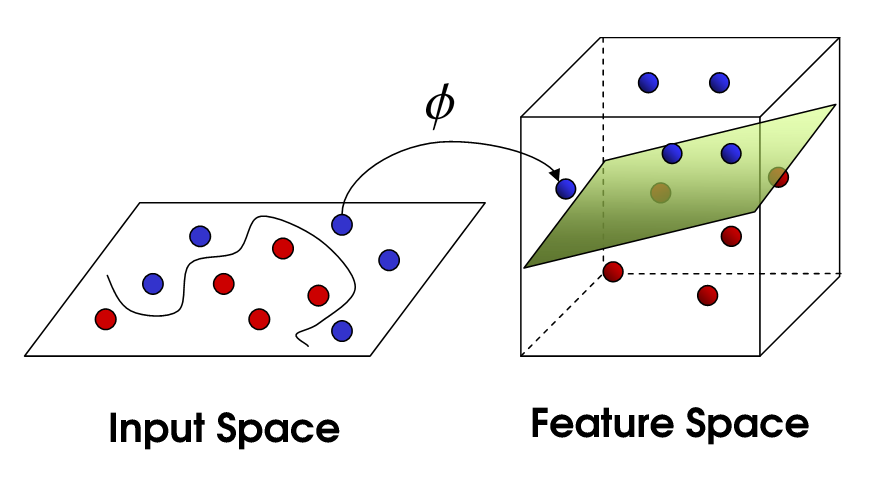
\includegraphics[scale=0.4]{Figures/phi}
    \caption{A visual rendition of the $\phi$ function, mapping samples from the
    input feature space to another feature space of higher dimensionality so that
    they could become linearly separable (from \cite{rtesselli}).}
    \label{fig:phi}
\end{figure}

Given these premises, and a value of $M$ high enough for the mapped samples to
be linearly separable, a kernel machine looks for the optimal linear separator in
$\mathcal{H}$ that corresponds to a non-linear separator in the input space.
To find this optimal separator the kernel machine has to deal with samples of
very high (possibly infinite) dimensionality and this could quickly render the
search for the solution to the optimization problem infeasible or too onerous.
Given that in the problem formulation the function $\phi$ only appears inside
the computation of dot products, values can be calculated by a kernel
function (section~\ref{subsec:kernelfunc}) thus referring to $\mathcal{H}$
only implicitly and avoiding to deal with a high number of dimensions
altogether using what is commonly known as the \emph{kernel trick}.

\subsubsection{Support Vector Machines}
\label{subsubsec:svm}
Here we will briefly describe one of the most tried kernel machines in the literature. 
\emph{Support Vector Machines} or SVM \cite{Cortes&Vapnik:1995} rest on the principle of structural risk
minimization (Section \ref{subsec:srm}) providing a trade-off between hypotheses
space complexity and the performances in fitting the training data.
It is a binary classifier but can be used to solve multi-class classification
problems with some additional work to combine multiple instances of this binary
classifier.
It is also a linear classifier and can be easily extended to the 
non-linear domain by using it in conjunction with (non-linear) kernel functions.
Given a feature space, this method tries to find the optimal hyperplane that
correctly separates the samples in such space, and separates them in the
most general way that is, maximising the \emph{margin} between each class.
In order to minimize the bound on true error (Section \ref{subsec:srm})
this method uses hypotheses spaces of crescent VC-dimension, to minimize the
VC-confidence while keeping a low empirical error.
There are two main settings in which this algorithm can work: when the data
is linearly separable in its original feature space and when it is not.
In the first case, since the empirical risk is going to be zero, finding the
optimal hyperplane means finding the one that again minimizes the VC-dimension
which in turn is the one that maximizes the margin between the classes i.e.
the minimum distance between the hyperplane and the nearest sample.
Solving this problem equals to solving the following quadratic optimization
problem:

\begin{gather}
    \begin{aligned}
        & min_{\vec{w},b}\frac{1}{2}||\vec{w}||^2 \\
        & \text{s.t. } \forall i \in \{1,\dots, n\} : y_i(\vec{w}\cdot\vec{x_i} + b) - 1 \geq 0 
        \label{eq:lsvm}
    \end{aligned}
\end{gather}

where $\vec{w} \cdot \vec{x} + b$ defines the hyperplane.
Since the margin we are looking to maximize is inversely proportional to the norm
of $\vec{w}$, we want to minimize the latter while the $\frac{1}{2}$ factor stems
from mathematical convenience.
Equation \ref{eq:lsvm} shows the primal form of the problem, whose formulation
has a convex cost function and constraints, hence it can be solved more easily 
switching to its dual form that, given these premises, will have the same
optimal solution.
Thanks to the Kuhn-Tucker theorem we can formulate the dual form using
Lagrange's multipliers:

\begin{gather}
    \underset{\vec{w},b}{\mathrm{min}}\,\underset{\vec{\alpha}\geq 0}{\mathrm{max}}\,L(\vec{w},b,\vec{\alpha})
    \label{eq:ldual}
\end{gather}

where $L$ is the lagrangian function and $\vec{\alpha}$ the multipliers.

\begin{equation}
    L(\vec{w},b,\vec{\alpha}) = \frac{1}{2}||\vec{w}||^2 - \sum_{i=1}^n \alpha_i(y_i(\vec{w}\cdot\vec{x} + b) - 1)
    \label{eq:lagrange}
\end{equation}

The optimal solution of this problem is the saddle point obtained while minimizing
w.r.t. $\vec{w}\text{ and }b$ and maximizing w.r.t. $\vec{\alpha}$.

When reaching this point the gradient of the function $L$ must be null:

\begin{gather}
    \begin{aligned}
        & \frac{\delta L(\vec{w},b,\vec{\alpha})}{\delta\vec{w}} = 0 \iff \vec{w^*} = \sum^{n}_{i=1} y_i\alpha^*_i\vec{x_i}\\
        & \frac{\delta L(\vec{w},b,\vec{\alpha})}{\delta b} = 0 \iff \sum_{i=1}^{n} y_i\alpha^*_i = 0\\
        & \alpha^*_i[y_i(\vec{w^*}\cdot \vec{x_i}+b^*) - 1] = 0,\,i=1,\dots,n
        \label{eq:lagrangedual}
    \end{aligned}
\end{gather}

and this lets us get rid of the primal variables in the lagrangian function since
they can be expressed using the labelled samples and the multipliers hence
reducing the problem to the maximization of $L(\vec{\alpha})$.
Those samples $X_i$ for which the $\alpha^*_i$ are greater than zero are called
support vectors and are the ones closer to the hyperplane, determining the margin,
as can be seen in Figure \ref{fig:slacks}.

The other case, that is when the data is not linearly separable, is solved in a
similar way but with the introduction of \emph{slack variables}, one for each
constraint:

\begin{equation}
    y_i(\vec{w}\cdot\vec{x} + b) \geq 1 - \xi_i
\end{equation}

These variables $\xi_i$, will account for the constraint violations by modifying the cost
function:

\begin{equation}
    \frac{1}{2}||\vec{w}||^2 + C \sum_{i=1}^n \xi_i
\end{equation}

where $C$ is a regularization parameter that will balance the trade-off between
the hypotheses space complexity and the number of non-separable samples.
Recalling the dual form of the previous case after the elimination of the primal
variables from the lagrangian function (Equations \ref{eq:lagrange} and \ref{eq:lagrangedual}),
we can now formulate our problem in the following way:

\begin{gather}
    \begin{aligned}
    & \underset{\vec{\alpha}}{\mathrm{max}} \sum_{i=1}^n \alpha_i - \frac{1}{2} \sum_{i,j=1}^n y_iy_j\alpha_i\alpha_j\vec{x_i}\vec{x_j}\\
    & \text{s.t. } \forall i \in \{1,\dots, n\} : 0 \leq \alpha_i \leq C,\, \sum_{i=1}^n y_i\alpha_i = 0 
    \end{aligned}
\end{gather}

This formulation differs from the previous one in that the dual variables (the $\alpha_i$s)
have $C$ as an upper bound.
The role of the slack variable $\xi_i$ is exemplified in Figure \ref{fig:slacks}.

\begin{figure}[ht]
    \centering
    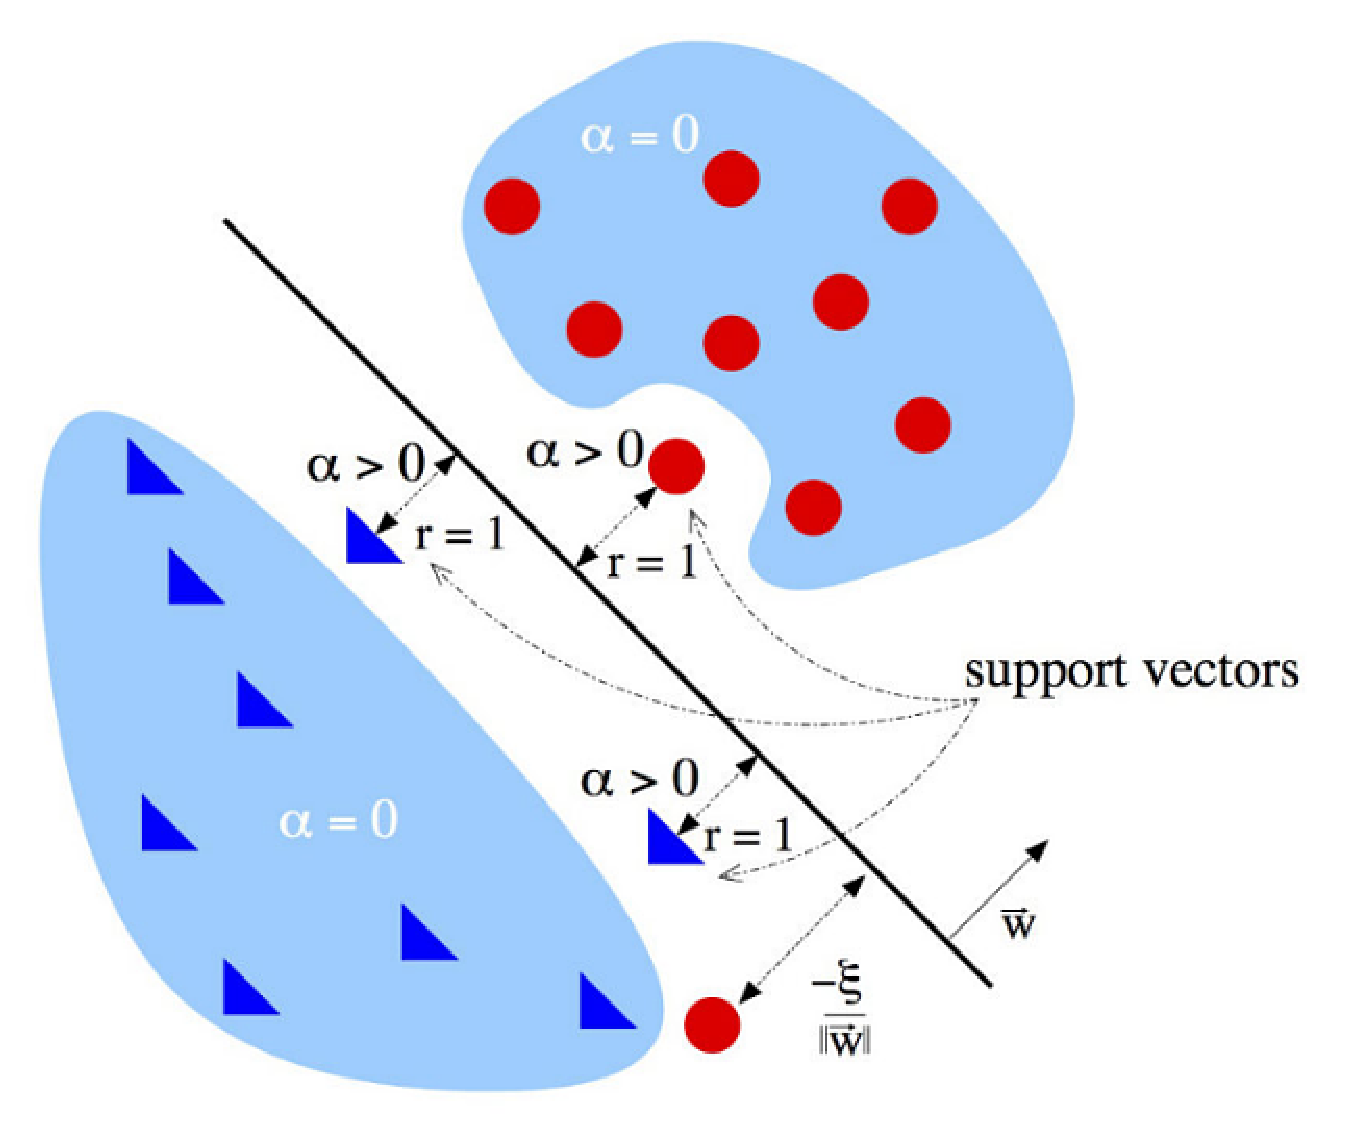
\includegraphics[scale=0.4]{Figures/slacks2}
    \caption{Effect of the introduction of \emph{slack variables} ($\xi$) in the SVM
    formulation variant known as \emph{soft margin} SVM.}
    \label{fig:slacks}
\end{figure}

The above approach has the major drawback that cannot guarantee good performances
in highly non-separable data because of the limitation in the ways an hyperplane
can separate any feature space, i.e. through dichotomies.
A remedy to this fact is to use the technique exposed in Section \ref{subsec:kmachines}
while maintaining the same formulation explained above where the dot product between
the samples in the (mapped) feature space is substituted with the kernel value on the
same samples.
The effects of this technique on the classification task is visible in Figure \ref{fig:kernsvm}.

\begin{figure}[ht]
    \centering
    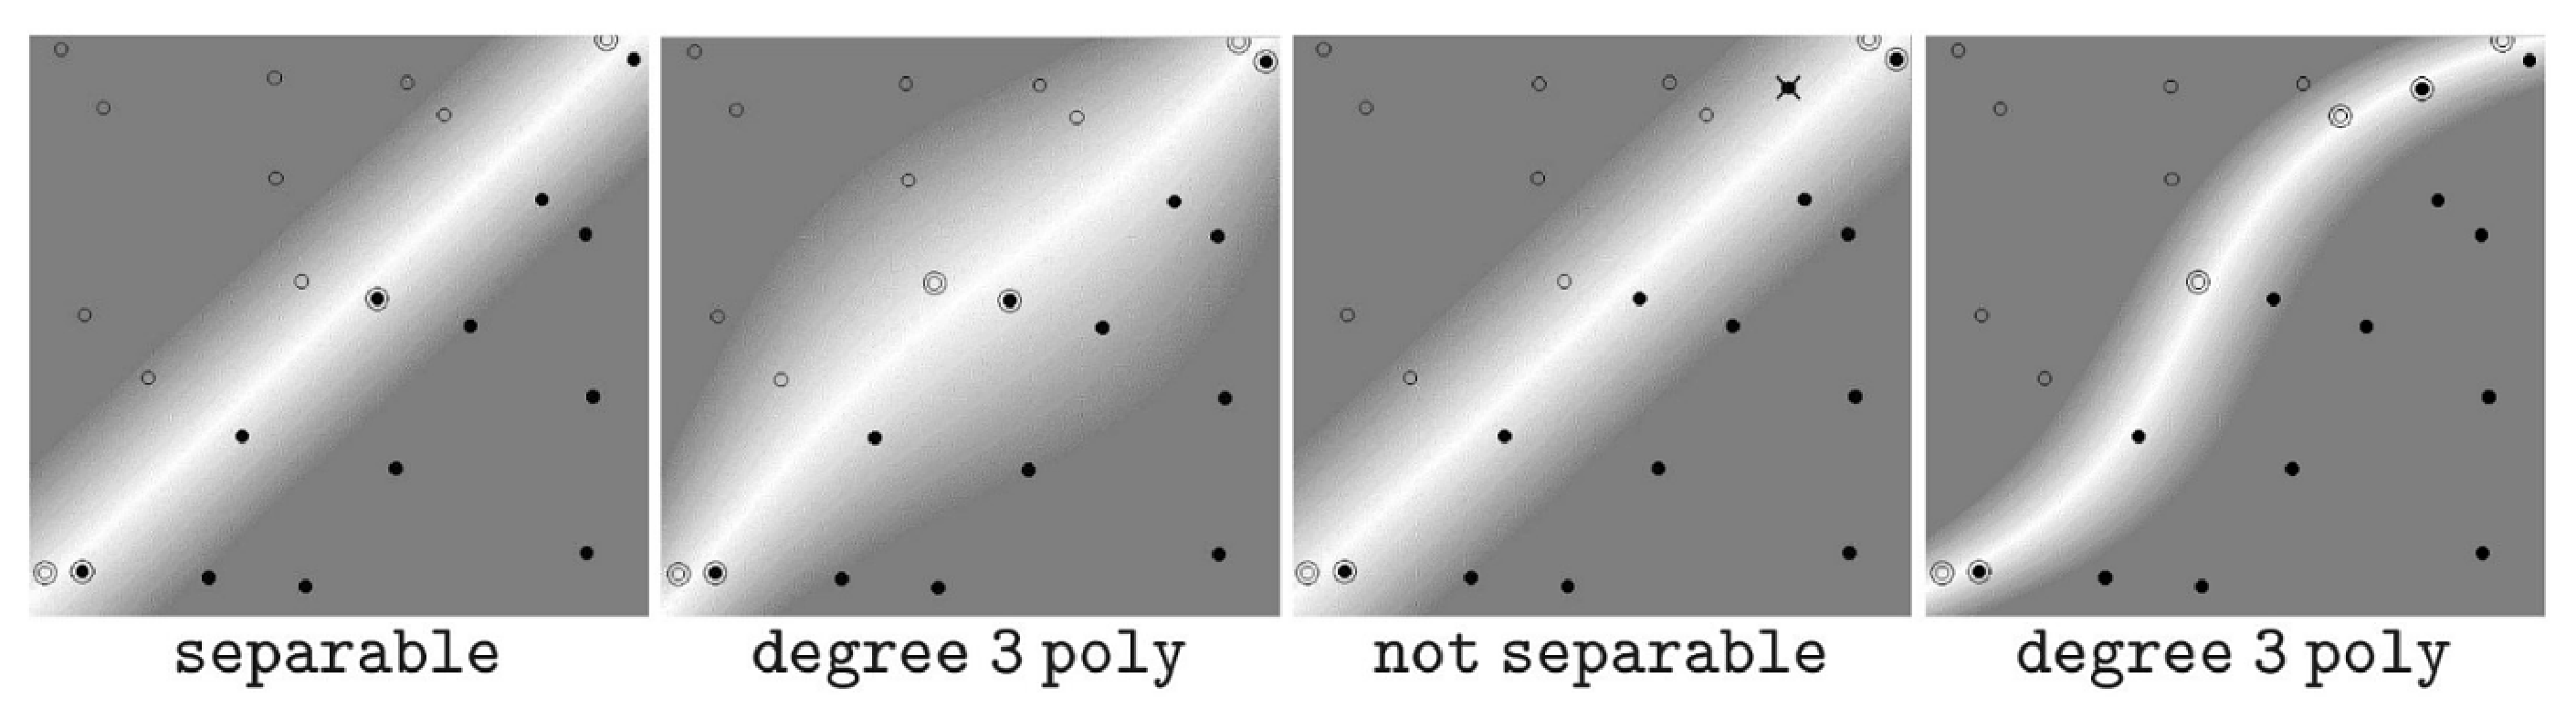
\includegraphics[scale=0.3]{Figures/kernsvm}
    \caption{Different effects on the decision surfaces generated on the input
        feature space without (first and third pictures) and with kernel (second and last pictures)
        in the two cases where data is linearly (first two pictures) and non-linearly separable (last two pictures)
        [ref lecture slides].}
    \label{fig:kernsvm}
\end{figure}

%----------------------------------------------------------------------------------------

\section{Kernels for structured data}
\label{sec:graphkernels}

In the previous section we introduced the theoretical foundations behind kernel
functions and the related learning methods.
The kernel learning approach is certainly convenient, the user needs to concentrate
its effort on the selection or design of the right kernel function for the problem
at hand, then couple it with one of the available general-purpose learning algorithms to
get a full-fledged learning method.
That being said, it is clear that in this scenario the kernel function is the
component responsible for the main source of bias.
Nowadays a number of different kernel functions are available with varying degree
of complexity in order to deal with a variety of problems, most of which has data
represented in vectorial form.
The rise of problems where data is naturally better represented with a
structured form (Section \ref{subsubsec:examples}) has rendered necessary the
study of new methods to tackle them.
One way of working with structured data could be to actually get rid of the structure
deriving an \emph{ad-hoc} vectorial representation, in what is called a
\emph{structure-based} approach.
This method is expensive and cumbersome since it forces the user to have a strong
knowledge of the task domain and to re-develop a new vectorial representation
for each task that she may encounter.

A more effective approach would be to adapt the methods to work directly on
structured data, and in this regard kernel methods are a good fit since the
decoupling between the kernel function and the kernel machine leaves the
only contact point between the data and the method in the function itself.
These methods maps the sample instances into high dimensional vectors and do it
in a general way without any knowledge of the underlying data beside its structure.
Furthermore this mapping is done implicitly meaning that they also have an
advantage from a computational standpoint.

Designing such kernel functions that can deal with structured data is a process
that has to balance between designing functions that are expressive enough to
produce some learning and the computational efficiency that it is required in
order to effectively perform the learning process.
As an example of this trade-off consider a kernel on graphs that counts all the
matching subgraphs between two input graphs.
This is certainly one of the most expressive possible kernels if not the most expressive
at all.
Even if such enumeration would exist, the kernel would still need to solve the
subgraph isomorphism problem several times, but that is clearly infeasible since subgraph
isomorphism is NP-hard.
Algorithmic complexity for a kernel function is a major point since the kernel has
to be computed for each pair of samples, rendering even a quadratic complexity
a hindering factor for its application.

A theoretically grounded way to design efficient and effective kernel functions for
structured data has been proposed by Haussler \cite{haussler99convolution} and
it is explained in the next section.
The main concept behind his work is that we need to restrict the number and type
of features considered for each structure.
Again, the choice of the substructures that would become features deeply affects
the learning outcome and is one of the major sources of bias in the whole learning
process, possibly leading to greatly differing performances according to different
datasets.
For what concern the scope of this thesis we will see in the following sections
some examples of kernels defined on trees and on graphs, all of which are instances
of the framework proposed by Haussler.

\subsection{The framework: convolution kernels}
\label{subsec:convolution}
Haussler's work \cite{haussler99convolution} main result is the \emph{R-convolution} framework,
a method for defining positive definite kernel functions on any object provided that a
positive semidefinite kernel for some decomposition of that object is available.
To give a brief formalization of the main idea, let $\mathcal{X}$ be a space of 
objects such that $x \in \mathcal{X}$ is associated with a finite subset
$\mathcal{X'_\mathit{x}}$ of some space $\mathcal{X'}$.
Assuming that: a kernel $k: \mathcal{X'}\times \mathcal{X'} \to \mathbb{R}$ is
defined and a \emph{finite} relation $R \subseteq \mathcal{X'}^D \times \mathcal{X'}$
is defined, we can now define an $R-convolution$ kernel:

\begin{equation}
    K(x,y) = \sum_{(x'_1,\dots,x'_n,x) \in R} \Bigg(\sum_{(y'_1,\dots,y'_n,y) \in R}
    \prod_{i=1}^D k(x'_i,y'_i)\Bigg)
\end{equation}

that, with the commonly used formulation with $D=1$ becomes:

\begin{equation}
    K(x,y) = \sum_{(x',x) \in R} \sum_{(y',y) \in R} k(x'_i,y'_i)
\end{equation}

Haussler was able to demonstrate the positive semi-definiteness of any kernel $K$
thusly defined, provided that $k$ is also positive semi-definite.

This work has later been extended and generalized \cite{Shin2010} with the introduction
of the \emph{mapping} kernel of which the \emph{R-convolution} kernel is a corollary.
This more general framework defines a mapping set
$M_{x,y} \subseteq \mathcal{X'_\mathit{x}} \times \mathcal{X'_\mathit{y}}$ and a \emph{base kernel} $k$ on it
that will hence consider only a subset of the entire cross product $\mathcal{X'_\mathit{x}} \times \mathcal{X'_\mathit{y}}$.
With these premises, a mapping kernel is defined as:
    
\begin{equation}
    K(x,y) = \sum_{(x',y') \in M_{x,y}} k(x',y')
\end{equation}

The positive semi-definiteness of the kernel $K$ is guaranteed only if the
mapping $\{M_{x,y}|x,y \in \mathcal{X}\}$ is transitive.
In the following sections we will analyse some of the latest contributions in terms
of kernel on structured data namely tree kernels and graph kernels.

\subsection{Kernels For Trees}
This family of kernels stems directly from the convolution kernel and each one
works by defining a different decomposition for the input tree.

\subsubsection{Subtree kernel}
\label{subsubsec:st}
The feature space of this kernel is composed of all the proper subtrees of the
input tree.
Let $X$ and $Y$ be two trees, the  subtree kernel is defined as:
\begin{equation}
    K_{ST}(X,Y) = \sum_{x \in X} \sum_{y \in Y} \delta(x,y)w_x =
    \sum_{s \in \mathcal{A}^*} h_s(X)h_s(Y)w_s
\end{equation}

where $x$ and $y$ are proper subtrees of $X$ and $Y$ respectively, $w_x$ is the 
weight associated with the tree $x$, $\mathcal{A}^*$ is the set of all the possible
subtrees, $h_s(X)$ counts the frequency with which $s$ appears in $X$ and
$\delta$ is the Kronecker's delta function, a function that evaluates to 1 if its
arguments matches, 0 otherwise.
The complexity of this formulation is indeed quadratic but in practice it can be
lowered to $O(nlogn)$, $n$ being the maximum number of nodes in either $X$ or $Y$,
using suffix trees \cite{viswanathan04fastkernels}.

\subsubsection{Augmented subtree kernel}
A more discriminative version of the previous kernel is the \emph{augmented} version
which extends the feature space of the subtree kernel with new features.
Usually adding more feature has an impact on the computational side of a kernel,
in \cite{dasanmartino2015exploiting} however an extension called ST+ kernel has been proposed with
only a modest increment in computational time.
Given a tree $T$, this kernel considers at most $\rho(v)h + 1$ features for any
$v \in V_T$ which are:
\begin{itemize}
    \item the proper subtree rooted at $v$, $\overset{v}{\triangle}$;
    \item for every $j^{th}$ child of $v$, $ch_v[j]$, and for every $l\text{ s.t. }0 \leq l < h$,
        the subtree of $T$ composed by:
        \begin{itemize}
            \item $v$ as root,
            \item $\overset{ch_v[j]}{\triangle}$,
            \item $T_{l-1}(ch_v[i],T) \forall i \in children(v), i \ne j$.
        \end{itemize}
\end{itemize}

An example of feature extraction is given in Figure \ref{fig:featext}.

\begin{figure}[ht]
    \centering
    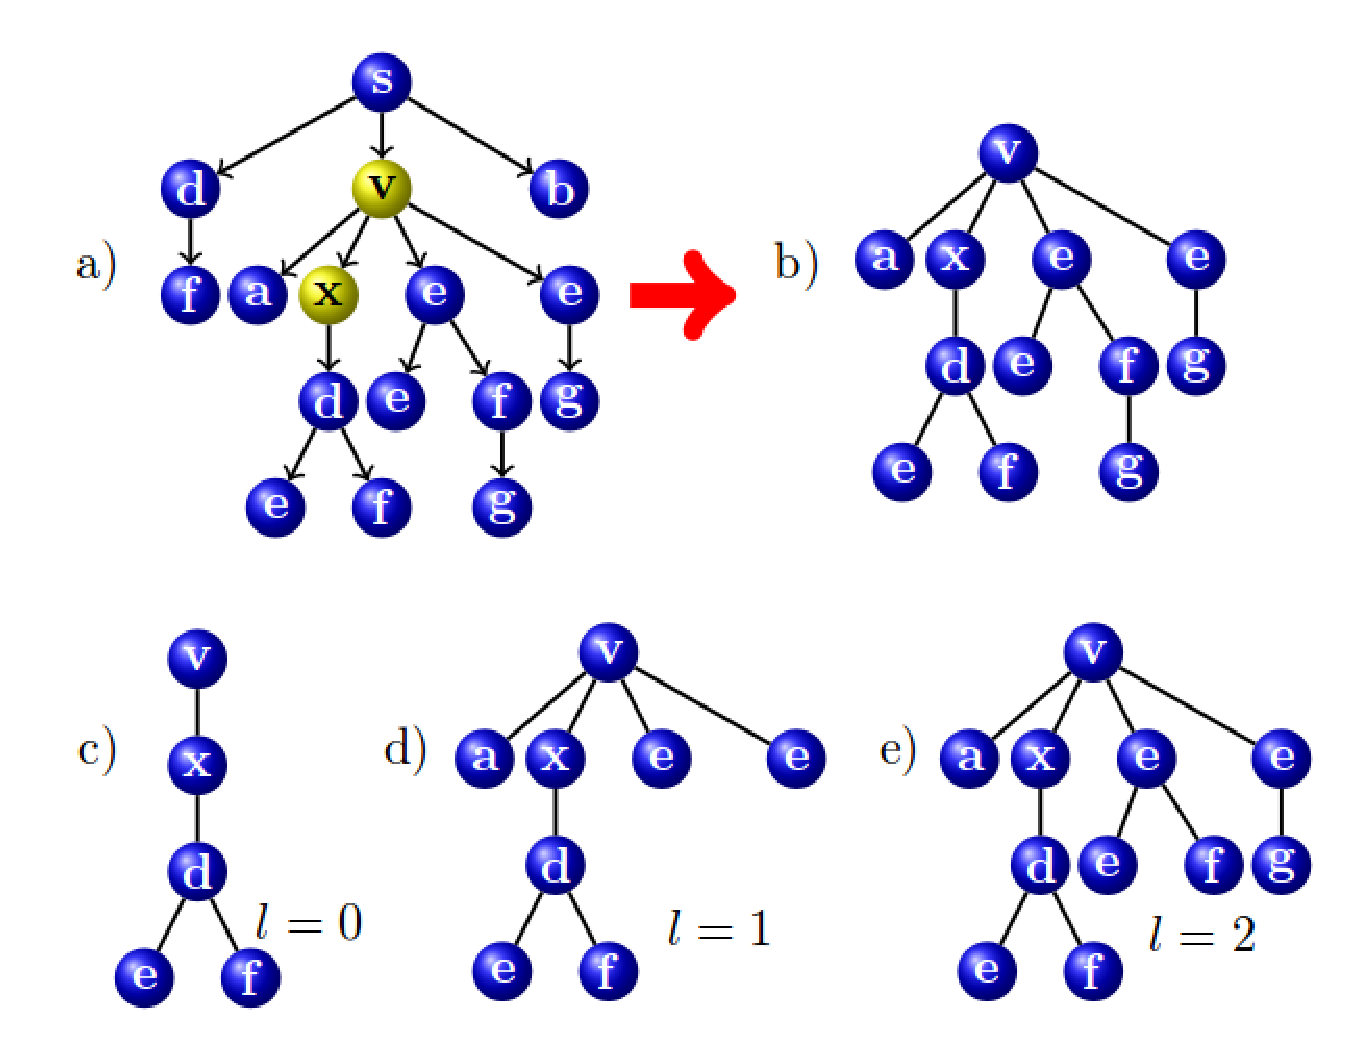
\includegraphics[scale=0.4]{Figures/featext}
    \caption{Feature space representation related to the kernel ST+ for an example
    tree: a) the input tree; b) the proper subtree rooted at the node labelled as $v$;
    c)-e) given the child $x$ of $v$, the features related to visits limited to $l$ levels (from \cite{dasanmartino2015exploiting}).} 
    \label{fig:featext}
\end{figure}

The formulation of this kernel is the following:

\begin{equation}
    K_{ST+}(T_1, T_2) = \sum_{s=1}^m h_s(T_1)h_s(T_2)
\end{equation}

where $m$ is the number of distinct trees corresponding to ST+ features, extracted
from a finite set of trees, and $h_s(T)$ the number of times the feature $t_s$
appears in $T$.

The proposed implementation in \cite{dasanmartino2015exploiting} has a complexity of
$O(Hh^2\rho^2log\rho)$ with $h$ and $H$ being the limit
of the tree visit and the number of nodes of that tree respectively.

\subsection{Kernels For Graphs}

As previously mentioned, defining kernels on graph is a challenging task, mainly
because of the need to balance the trade-off between the expressiveness of the
feature space and the computational effort needed for feature extraction and
kernel calculation.
Expressive kernels are usually well performing in terms of predictive power but
are also typically more expensive to compute.
On the other hand a less discriminative kernel is usually easier to calculate
at the expenses of some learning power.
To further explain this point, consider the class of kernels that are able to
distinguish between all the (non-isomorphic) graphs in the feature space.
Being able to distinguishing between two non-isomorphic graphs that belongs to two
different classes is essential for any machine learning approach.
However, computing such kernel in an efficient way would equals to solve the
graph isomorphism problem in a similarly efficient way and this is not the case
since at the moment there are no polynomial time algorithms for solving the graph isomorphism problem.
Another interesting group of kernels is the one that given a graph $X$, it decomposes
it into the set of its subgraphs and maps it to a set of features $\phi_h$ that, for
each graph $h$ measure how many subgraphs of $X$ are isomorphic to $h$.
Again this class of kernels has to deal with the solution of the same NP-hard
problem explained above, so probably no such efficient kernel exists.

Recent research has focused on the study and development of less expressive
kernels that have the major advantage of being computable in polynomial time.
In the following sections we will briefly discuss the kernels that falls in the
scope of the present thesis, and give an overview of the recent improvements that
have been proposed in the literature.

\subsubsection{ODD kernels}
\label{subsubsec:odd}

Before the introduction of the ODD kernel framework, a number of graph kernels
could already be found in literature, such as the \emph{random walk kernels} \cite{Gaertner04mlj},
the \emph{subtree pattern kernel} \cite{ramon03graphkernels}, and the \emph{shortest path kernel}
\cite{borgwardt05graphkernel}, but they remained computationally very onerous, with
the first family having polynomial complexity only on undirected graphs, the second one
having exponential complexity and the last one being more than quadratic.
The \emph{ODD kernel framework} proposed in \cite{DBLP:conf/sdm/MartinoNS12} aims
to be a kernel framework that can be instantiated with the right trade-off between
expressiveness and efficiency for different tasks.
The original work presents an instantiation with the ST kernel, while another
recent work \cite{dasanmartino2015exploiting} instances the framework to an adaption
of the ST+ kernel.

The Ordered Decomposition DAG Kernels framework (ODDK) basically decomposes the
graphs in a set of simpler trees, where it is easier to compute the isomorphism
using efficient tree kernels.
The framework consists of these steps:

\begin{enumerate}
    \item the input graph $g$ is mapped into a multiset of decomposition DAGs\\
        $\{DD_g^{v_i}|v_i \in V_g\}$; $DD_g^{v_i}$ is obtained from its root $v_i$
        and the edges that appear in the shortest paths from $v_i$ to any other node
        $v_j \in V_g$;
    \item a strict partial order on the vertices of the DAG has to be defined
        to make an unique representation of the subtrees possible.
    \item each Ordered Decomposition DAG $ODD_g^{v_i}$ thus obtained that is, each
        decomposition DAG with the nodes ordered according to the partial
        order relation defined above, is then mapped into
        one or more trees $T(v_i,ODD_g^{v_i})$, where $T(\cdot,\cdot)$ is the function
        that returns the tree resulting from the tree visit on $ODD_g^{v_i}$ starting
        from node $v_i$, and the kernel between two graphs $g_1$ and $g_2$ is
        defined as:
        \begin{equation}
            ODDK(g_1,g_2) = \underset{OD_2 \in ODD_{g2}}{\underset{OD_1 \in ODD_{g1}}{\sum}}
            \sum_{j=1}^h\sum_{l=1}^h
            \underset{v_2 \in V_{OD_2}}{\underset{v_1 \in V_{OD_1}}{\sum}}
            C(r(T_j(v_1,OD_1),r(T_l(v_2,OD_2)))
        \end{equation}
        where $C$ is the function defined by the chosen tree kernel.
\end{enumerate}

Considering the instantiation of the framework with the ST kernel and limiting
the size of the tree-visits $T_j(v_1)$, with the $h$ parameter that regulates the
maximum height of the considered substructures, and by assuming $\rho$ constant
the time complexity of $ODDK$ with ST features is $O(|V_g|log|V_g|)$.

\subsubsection{Fast subtree kernels}
\label{subsubsec:fs}
The fast subtree kernel \cite{NIPS2009_3813} belongs to family of kernels defined
as instances of the Weisfeiler-Lehman kernel framework which bases its discriminative
power on the Weisfeiler-Lehman test of isomorphism.
The main idea behind this framework is that every graph can be represented as
a sequence of graphs, each one being generated from the previous one through
a new labeling function that encapsulates the isomorphism test.
Given a graph $X = (V,E,L)$, this sequence can be formally defined as:

\[\{X_0,X_1,\dots,X_h\} = \{(V,E,L_0),(V,E,L_1),\dots,(V,E,L_h)\}\]

where $X_0 = X$, $L_0 = L$ and $L_i$ is represents the relabeling of the graph
$X_{i-1}$ obtained applying the Weisfeiler-Lehman test.

Let $k$ be a positive semidefinite kernel for graphs the Weisfeiler-Lehman kernel
framework can be formulated as:

\begin{equation}
    K_{WL}^h(X,Y) = k(X_0,Y_0) + k(X_1,Y_1) + \dots + k(X_h,Y_h)
    \label{eq:fs}
\end{equation}

A first instance of this framework is the \emph{Weisfeiler-Lehman subtree kernel}
($WL$) which considers all the subtree patterns up to height $h$ and checks whether the
neighbourhoods of two nodes match exactly.
To define this kernel it is sufficient to define the base kernel for Equation
\ref{eq:fs} as:

\begin{equation}
    k(X,Y) = \sum_{x \in V(X)}\sum_{y \in V(Y)} \delta(L(x),L(y))
    \label{eq:wl}
\end{equation}

where $\delta$ is again the Kronecker's function.

With the base kernel defined in Equation \ref{eq:wl}, $K_{WL}^h$ becomes the
kernel defined in \cite{NIPS2009_3813}.

\subsection{Latest Improvements on Graph Kernel Methods}
\label{subsec:kernel}
In the recent years a number of improvement over the above mentioned kernel approaches
have been proposed, mainly to try to improve the expressiveness of the feature
spaces without incurring in major computational drawbacks.
Among the others, and mainly because inside the scope of this thesis we will
mention in no particular order:
\begin{itemize}
    \item the addition of contextual information \cite{Navarin2015},
    \item the extension of the $ODD_{ST}$ kernel to employ an MKL approach,
    \item the extension and generalization of the Weisfeiler-Lehman framework \cite{SanMartino2014}.
\end{itemize}

The next section will give a brief overview of the first point while in section
\ref{subsec:gmkl} we will delve a bit more in detail in the MKL approach
with respect to graph kernel learning.

\subsubsection{Kernels with contextual information}
\label{subsec:context}

The kernels described in the previous section try to approximate complex
structures by the means of decomposing them in simpler substructures on which
define a measure of similarity.
Even though they employ different type of substructures, they have in general
similar predictive performances.
A recently proposed work \cite{Navarin2015} on graph kernels, aims to improve local
feature expressiveness by enriching the feature space with contextual information,
that is, a description of the topology of the graph around the extracted feature.
The cited work proposes an extension of the $ODD_{ST}$ kernel, derived from
\cite{rtesselli} where extensions of the $ODD_{ST+}$ kernel ($TCK_{ST+})$ and of the $WL$
kernel ($WLC$) are proposed.
In this way an increase of discriminative power is expected, since two identical
features need also to appear in the same context within two graphs to match.
Therefore a feature contribution is built up by the contribution determined by
its contexts. To express it more formally, given a graph $g$ and a feature $f$
the following property holds from \cite{Navarin2015}:

\begin{equation}
    \phi_f(g) = \sum_{c \in Contexts_g(f)} \phi_{f\circ c}(g)
\end{equation}

where $\phi_f(g)$ is the frequency of the feature $f$ in the RKHS of the original
kernel and $\phi_f\circ c(g)$ is the frequency of the it appearing within the
context $c$.

Given the parent-child relationship between contexts and features, it is
straightforward to see that they can share the same representation, i.e. the
context is a substructure of the graph that contains the feature.
This leads to the useful facts that context can be feature themselves and that to
compute contextualized features it suffices to combine features with other
features representing contexts.
The Tree Context Kernel can thus be defined as:

\begin{gather}
    \begin{aligned}
        TCK(G_1,G_2) &= \underset{v_2 \in V_{G_2}}{\underset{v_1 \in V_{G_1}}{\sum}}
        \sum_{i=1}^h\sum_{j=1}^h
        ~[\delta(T_i(v_1,G_1),T_j(v_2,G_2))\\
            &+\underset{\overset{u_2}{\triangle} \in T_i(v_2,G_2)}{\underset{\overset{u_1}{\triangle} \in T_i(v_1,G_1)}{\sum}}
        \delta(\overset{u_1}{\triangle},\overset{u_2}{\triangle})
    \sum_{l=1}^{\rho(u_1)} C_{ST}(ch_l(u_1),ch_l(u_2))]
    \end{aligned}
\end{gather}

%where:
%
%\begin{equation*}
%    C_{ST}(v_1,v_2) = 
%        \begin{cases}
%            \lambda \cdot K_L(v_1,v_2) & \text{if } v_1 \text{ and } v_2 \text{ are leaves} \\
%            \lambda \cdot K_L(v_1,v_2)\,\prod_{j=1}^{\rho(v_1)} C_{ST}(ch_j(v_1),ch_j(v_2)) & \text{if } \rho(v_1)=\rho(v_2) \\
%            0 & \text{ otherwise}
%        \end{cases}
%\end{equation*}

where $\delta$ is the Kronecker's function, $h$ is the user defined depth limit of 
the tree-visit and $C_{ST}$ is the function related to the ST kernel (see Section \ref{subsubsec:st}) that counts the common
subtrees of the two trees rooted at $v_1$ and $v_2$.

In more simple terms the kernel will score a match in the following cases:
\begin{itemize}
    \item both $v_1$ and $v_2$ are root nodes of the tree visit, i.e. $u_1 = v_1$ and $u_2 = v_2$
    \item $v_1$ and $v_2$ appear within the same context in both the trees
\end{itemize}

This kernel is provably positive semidefinite because it is a combination of positive
semidefinite kernels (see the end of Section \ref{subsec:convolution}).

\section{Multiple Kernel Learning}
\label{subsec:mkl}
Multiple Kernel Learning aims to enhance the accuracy of a target kernel machine
combining kernels derived from multiple sources in a data-driven way.
The rationale behind this idea is similar to the one behind classifier combinations.
Instead of deciding a priori which kernel to use, it is better to devise an
algorithm that can either choose for us or better, learn a combination of the
possible choices.

Hence MKL can be used to mitigate the bias deriving from a single kernel choice
or to combine different source of information that rely on different data representation
thus requiring a number of different kernels.

Furthermore it relieves the final user from the often arduous task of designing
a strong kernel by allowing her to implement a number of more ``weak'' kernels
that can work in combination to perform the learning task.

The available methods in the literature can be summarily divided in two categories
\cite{journals/jmlr/GonenA11}: on one hand \emph{fixed rule} algorithms which as the name implies apply some fixed
rule or heuristic to determine the combination parameters, thus being able to scale
well with respect to the number of kernels but whose effectiveness is bounded by
the effectiveness of the rule on the domain being considered,
on the other hand, \emph{optimization based} approaches solve an optimization
problem to derive their combination parameters.

There are two fundamental ways to use the MKL approach: combine a small set of 
relatively strong and carefully designed kernels, a method which has shown no
significant improvement over a simple combination like the averaging of the kernels;
then the converse, combine a large set of weak kernels aiming at boosting their
individual performances exploiting a data driven rather than an expert driven
approach.

In the following section we will give an overview of the MKL implementation
that we chose for the present work.

\subsection{EasyMKL}
\label{subsec:easymkl}

The method proposed in \cite{aiolli2015easymkl} focuses on the linear positive combination
parameters version of MKL which can be formulated as

\begin{equation}
    K = \sum_{r=1}^R \eta_rK_r,\, \eta_r \geq 0
    \label{eq:easymkl}
\end{equation}

The goal is to learn a vector of coefficients $\vec{\eta}=\{\eta_r\}_{1\leq r \leq R}$ that will form the
combined kernel according to Equation \ref{eq:easymkl}.
The proposed algorithm can be ascribed to the category of optimization based
techniques since in it requires the solution of an optimization problem whose
formulation follows:

\begin{equation}
    \underset{\vec{\eta}:||\vec{\eta}||=1}{\mathrm{max}}\underset{\gamma \in \hat{\Gamma}}{\mathrm{min}}(1-\Lambda)\gamma^\top\hat{Y}\Big(\boldsymbol{\sum_r^R \eta_r\hat{K_r}}\Big)\hat{Y}\gamma+\Lambda||\gamma||^2
    \label{eq:easymin}
\end{equation}

where $\hat{K_r}\text{ and }\hat{Y}$ are the weak kernel computed on the training samples
and the training labels respectively, $\Lambda \in \{0,1\}$ is the regularization
parameter and $\gamma \in \hat{\Gamma}$ is the probability distribution over the set of positive and
negative training samples, $\hat{\Gamma}$ being the domain of probability distributions defined as:
\[ \hat{\Gamma} = \Big\{ \gamma \in \mathbb{R}^l_+ | \sum_{i \in \oplus} \gamma_i = 1, \sum_{i \in \ominus} \gamma_i = 1 \Big\} \]

This problem has a formulation similar to the one of the \emph{Kernel Optimization of the
Margin Distribution} algorithm (KOMD) \cite{Aiolli2008} where the kernel has been
substituted with the sum of the weak input kernels with the important implication
that the space requirements remain linear w.r.t. $R$.

In the margin maximization step of the algorithm, the $\Lambda$ parameter
has two critical points: when $\Lambda = 0$ there is no regularization so the
problem reduces to a hard margin SVM; when $\Lambda = 1$ the optimal solution is
the squared distance between the positive and negative centroids in the feature
space.
This is more evident looking at the experimental results in Chapter
\ref{Chapter4}.

\subsection{Multiple Kernel Learning On Graphs}
\label{subsec:gmkl}
A recent work \cite{gmkl} has managed to integrate the algorithm explained in the
previous section with the work on graph kernels conducted in \cite{DBLP:conf/sdm/MartinoNS12}.

The technique proposed in the paper aims to find a generalizable way of constructing
orthogonalized kernels starting from a single feature space, by the means of 
dividing the features in independent sets according to some strategy.

The work in \cite{gmkl} proposes a simple yet theoretically backed strategy that is,
the subdivision of the feature space of the $ODDK_{ST}$ kernel according to the
size of the features.
Given the inherent hierarchical structure of the tree features, dividing them by
height ensures that no two dependent features ends up in the same set.
Every set composed in this way is then used as a separate feature space to compute
a separate kernel and the whole list becomes the input for the EasyMKL algorithm.
An important point that emerges from this work is that, by using the MKL approach
in combination with an orthogonal partitioning of the feature space, a reduction
in the number of hyper-parameters to validate was obtained.
This latter point in particular it is a considerable addition to our proposed
methodology as explained in Section \ref{subsec:features}.

%----------------------------------------------------------------------------------------

% vim: spell spelllang=en_gb
 % Background
\chapter{Graph Kernels Combination}
\label{Chapter3}

This chapter details the contribution of the present work.
We start by analysing the motives behind kernels combination and in particular
behind graph kernels combination (section \ref{sec:why}).
Then, in the following sections, we proceed with examining the existing techniques
(section \ref{sec:tech}), we discuss in detail the proposed methodology (section
\ref{sec:meth}) and finally give an overview of the main optimization choices (sections
\ref{sec:opt}, and \ref{sec:inc})

\section{Why Combining Kernels}
\label{sec:why}

In the previous chapter we described a number of approaches (section \ref{sec:graphkernels})
and the relative improvements that has been presented in the recent years.

\subsection{The Case For Graph Kernels}

\section{Existing combination techniques}
\label{sec:tech}
%kernels SUM: descrption, pros, cons

\section{The Proposed Methodology}
\label{sec:meth}
%thorough description
 

This choice stem from the fact that the implementation we used for $MKL$ gives us
back a set of weights, one for each of the input kernel matrices; these weights,
multiplied by their related matrix which then get summed together give us the
best linear combination of the input kernels.
While a weight is not to be taken as an assessment of the goodness of a single
kernel matrix (since they are optimal as a combination), a very low weight can
indeed be a sure sign that the related matrix has given a very poor contribution
to the classification task.

% easyMKL altrimenti ciao

\subsection{Immersed Model Selection}
\label{subsec:parameters}
% butta tutte le matrici in un colpo solo
One of the main advantages of the proposed method is that it permits to embed
the otherwise cumbersome process of hyper-parameter optimization (section \ref{subsubsec:grid})
inside the learning phase in a completely transparent way, which will be hereby
described.

It is custom practice to perform hyper-parameter optimization employing a grid
search technique.
In our setting this would translate to having to compute one kernel matrix
for all the possible combinations of values deriving from every set of values
chosen for each parameter both from the kernel and the selected learning
algorithm, for instance the $h$ and $\lambda$ parameters for the $ODD$ kernels
and the $C$ parameter if using the SVM.
Then every thusly computed set of kernels would have been fed to the $MKL$
algorithm to be evaluated via cross-validation.
Let $l,m,n$ be the cardinality respectively of the three sets of values above,
the cross-validation instances would have been $l\cdot m\cdot n$.

A first improvement over the above scenario is to adopt a multiple kernel learning
approach and feed the algorithm the kernels computed from the grid all at once.
One of the advantages of this approach is that instead of selecting one combination
of parameters thus restricting the generalization power of the resulting model,
the whole set of parameters combination concurs in the model determination hence
increasing the chances of it being more general.

Given the fact that our $MKL$ implementation of choice has an algorithmic
complexity that is not dependent on the cardinality of the input but rather on
its dimensions, one drawback of this approach is that the memory consumption
invariably increases with the number of kernel thus making this approach still
computationally prone to the curse of dimensionality.

Section \ref{sec:opt} deals with a possible solution to this problem.

\subsection{Kernels and Feature Spaces}
\label{subsec:features}


% buckets => leva un parametro

%----------------------------------------------------------------------------------------

\section{Method optimization}
\label{sec:opt}
% memory consumption (+ alternate methods constant RAM)

Memory consumption is basically bound to $O(m\cdot n^2)$ with $m$ being the number of kernels and
$n$ the number of samples while being in practice $O(2\cdot (m\cdot n^2))$.
%----------------------------------------------------------------------------------------

\section{Incremental kernels calculation} 
\label{sec:inc}
The kernels we analysed in this study present feature space representations
that are in a subset relation; this prompted us to devise a method to calculate
such representations in an incremental fashion trying to gain a significant
speed-up.

\begin{algorithm}
    \caption{The devised algorithm to incrementally compute the explicit
    features space representation for the available ODD kernels, namely
    $ODD_{ST}$, $ODD_{STC}$, $ODD_{STP}$, $ODD_{STPC}$.}
    \label{alg:incremental}
    \begin{algorithmic}[1]
        \ForAll{$kernel \in Kernels$}
            \State $\phi_{kernel} \gets [0,\dots,0]$
        \EndFor

        \ForAll{$v \in V_g$}
            \State $f \gets \{\}$
            \State $size \gets \{\}$
            \State $dag \gets DAG_h(v, g)$
            \ForAll{$u \in \Call{ReverseTopologicalOrder}{dag}$}
                \ForAll{$d \in \{0,\dots,diam(dag)-|sp(v,u)|\}$}
                    \If{$d=0$}
                        \State $f_{u,0} \gets \kappa(L(u))$
                        \State $size_{u,0} \gets 1$
                        \State add $f_{u,0}$ to $\phi_{ODD_{ST}}$
                        \State add $f_{u,0}$ to $\phi_{ODD_{STP}}$
                    \Else
                        \State $(S_1,\dots,S_{\rho(u)}) \gets \Call{Sort}{
                        f_{ch_1(u),d-1},f_{ch_2(u),d-1},\dots,f_{ch_{\rho(u)}(u),d-1}}$
                        \State $f_{u,d} \gets \kappa(L(u)\lceil{}S_1\#S_2\#\dots\#S_{\rho(u)}\rfloor)$
                        \State $size_{u,d} \gets 1 + \sum_{i=1}^{\rho(u)}size_{ch_i(u),d-1}$
                        \ForAll{$ch \in children(u)$}
                            \State assign $f_{ch,d-1}$ as a context to $f_{u,d}$
                            \State compute weight of $f_{ch,d-1}$
                            \State add contextualized feature to $\phi_{ODD_{STC}}$
                            \State add contextualized feature to $\phi_{ODD_{STPC}}$
                        \EndFor
                        \State add $f_{u,d}$ to $\phi_{ODD_{ST}}$
                        \State add $f_{u,d}$ to $\phi_{ODD_{STP}}$
                    \EndIf
                    \If{$u=v$}
                        \State add $f_{u,d}\circ{}c$ to $\phi_{ODD_{STC}}$
                        \State add $f_{u,d}\circ{}c$ to $\phi_{ODD_{STPC}}$
                    \EndIf

                    \State Compute $ODD_{STP}$ and $ODD_{STPC}$ peculiar features
                    and contexts and add them to the relevant $\phi$ in a similar
                    fashion\label{line:stp}
                \EndFor
            \EndFor
        \EndFor
    \end{algorithmic}
\end{algorithm}

In Algorithm~\ref{alg:incremental}, line~\ref{line:stp} refers to the sub-procedures
defined in \cite{nnavarin, rtesselli}.
As one can see, given a graph instance, the algorithm is able to build and
collect the features in one pass thus maintaining a performance of $O(n)$ where
$n$ is the dimension of the input (i.e. the number of graphs) versus the
previous approach that would require $O(m \cdot n)$ with $m$ being the number of
kernels being computed.

\begin{figure}[ht]
    \centering
    \includegraphics[scale=0.4]{Figures/kernel_times}
    \caption{Times in seconds required to compute the kernels $ODD_{ST}$ and 
    $ODD_{STC}$ incrementally and sequentially on a selection of datasets.}
    \label{fig:times}
\end{figure}

The plot in figure~\ref{fig:times} shows the measured times on a variety of
datasets (see section~\ref{subsec:datasets} for further details on each one)

%----------------------------------------------------------------------------------------

 % Contribution
% Chapter 4

\chapter{Experiments}
\label{Chapter4}

In order to assess the quality of the proposed methodology we tested it on a
number of datasets and against a number of baselines that will be detailed in
the following sections.
Since our methodology has the parameter selection phase embedded in the learning
process (section~\ref{subsec:parameters}) the experiments structure were quite
straightforward, namely consisting in the pre-calculation of the relevant kernel
matrices, and then using them all at once in a stratified k-fold cross-validation
routine with the learning method of choice.
The $k$ parameter of the cross-validation has been fixed at 10 since this value
already provides good statistical significance while helping containing the bias
skewing during the training phase.
Moreover, the whole routine has been run ten times with ten different split of the
data to mitigate the high variance derived during the testing phase due to the
chosen value of $k$.

\section{Datasets}
\label{subsec:datasets}

The experiments were conducted on five real-world applications datasets, namely:
CAS \cite{cas}, NCI1 \cite{nci1}, AIDS \cite{aids}, CPDB \cite{cpdb}, and GDD \cite{gdd}.
All these datasets contains chemical and molecular particles encoded in graph form.
The AIDS Antiviral Screen dataset contains chemical compounds, categorized
into chemical groups; CAS and CPDB are dataset of mutagenic
compounds; NCI1 consists of chemical compounds screened for activity against 
non-small lung cancer cells; GDD is composed of X-ray crystal structures of
proteins represented as graphs.
The graph encoding of this data is such that every node is labelled and none
has a self loop that is there are no nodes with an edge going out and going back
into them.
Some statistics about these datasets are gathered in table~\ref{table:datasets}.

    \begin{table}[ht]
        \centering
        \begin{tabular}{|r|r|r|r|r|}
            \hline
            Dataset & n. of graphs & sample split & avg nodes & avg edges \\ \hline
            AIDS    & 1503         & 28.07        & 58.90     & 61.40     \\ \hline      
            CAS     & \textbf{4337} & 55.36        & 29.90     & 30.90     \\ \hline      
            CPDB    &  684         & 49.85        & 14.10     & 14.60     \\ \hline      
            GDD     & 1503         & 58.65        & 284.31    & \textbf{2862.63}   \\ \hline      
            NCI1    & 1503         & 50.04        & 29.87     & 32.30     \\ \hline      
        \end{tabular}
        \caption{Statistics about the datasets employed in the experiments: number
        of graphs, labels percentage among samples, average number of nodes, average
        number of edges. It is clear from this table that the CAS and NCI1 datasets
        are the bigger ones while the GDD holds the most complex graphs either in
        terms of topography and processing. Furthermore the AIDS dataset turns out
        to be quite unbalanced in terms of labels distribution \cite{rtesselli}.}
        \label{table:datasets}
    \end{table}

%----------------------------------------------------------------------------------------

\section{Experiments description}
\label{sec:description}

The original kernel combinations selected for this study were:
\begin{enumerate}
    \item the $ODDK_{ST}$ and $TCK_{ST}$ graph kernels,
    \item the $ODDK_{ST+}$ and $TCK_{ST+}$ graph kernels,
    \item the $WL$ fast subtree and $WLC$ graph kernels,
\end{enumerate}

for each combination a separated set of experiment was conducted, while maintaining
the same structure, of which a detailed breakdown will be given in Table \ref{table:structure}.

\begin{table}[ht]
    \centering
    \begin{tabular}{|l|l|l|}
        \hline
        exp. no. & method & kernels \\
        \hline
        1 & easyMKL & $K$ and $K'$ \\
        \hline
        2 & easyMKL & $K'$ \\
        \hline
        3 & easyMKL & $K$ \\
        \hline
    \end{tabular}
    \caption{Structure of the main experiments. Kernels $K$ and $K'$ refer
    to the version without and with contexts for each combination respectively.
    These kernels generated a set of matrices each, according to the technique
    described in Section \ref{subsec:features} which were concatenated as a list
    to be given in input to easyMKL.}
    \label{table:structure}
\end{table}

The hyper-parameter selection process for the kernels has been embedded
into the MKL learning phase so each set of kernel matrices has been
pre-computed for each one of the possible combination of parameters that would
otherwise have been used in a grid-search fashion.

\subsubsection[$ODDK_{ST}$ and $TCK_{ST}$]{$\boldsymbol{ODDK_{ST}}$ and $\boldsymbol{TCK_{ST}}$}
The kernels used for this experiment were generated from the $ODDK$ kernels
in \cite{odd, contexts}, namely $ODDK_{ST}$, $TCK_{ST}$.
Since EasyMKL took care of weighing the individual kernels, the $\lambda$
parameters of the ODD kernels has been fixed to 1, while the $h$ parameter
values were the set $\{1,\dots,10\}$.
During the cross-validation routine, the $\Lambda$ parameter of easyMKL has been
validated from the set $\{0.0, 0.1,\dots,1.0\}$.

\subsubsection[$ODDK_{ST+}$ and $TCK_{ST+}$]{$\boldsymbol{ODDK_{ST+}}$ and $\boldsymbol{TCK_{ST+}}$}
The kernels used for this experiment were generated from the $ODDK$ kernels
in \cite{stplus, rtesselli}, namely $ODDK_{ST+}$, $TCK_{ST+}$.
Again, EasyMKL took care of weighing the individual kernels so the $\lambda$
parameters of the ODD kernels has been fixed to 1, while the $h$ parameter
values were the set $\{1,\dots,10\}$.
During the cross-validation routine, the $\Lambda$ parameter of easyMKL has been
validated from the set $\{0.0, 0.1,\dots,1.0\}$.

\subsubsection[$WL$ and $WLC$]{$\boldsymbol{WL}$ and $\boldsymbol{WLC}$}
The kernels used for this experiment were generated from the $Fast~Subtree$ kernels
in \cite{fs, rtesselli}, namely the $WL$ kernel and the $WLC$ kernel.
These two kernels only need one hyper-parameter to validate, that is $h$ the iterations
limit whose chosen values were those in the set $\{1,\dots,10\}$.
During the cross-validation routine, the $\Lambda$ parameter of easyMKL has been
validated from the set $\{0.0, 0.1,\dots,1.0\}$.

\subsubsection{The GDD dataset}
\label{subsubsec:gdd}
Confirming the experience reported in \cite{contexts}, while working with the GDD
dataset and the $ODD$ kernels we had to limit the $h$ hyper-parameter to the set
$\{1,2,3\}$ because for heights greater than 3 the computational times of the
kernel matrices became prohibitive, due to the high complexity and magnitude
of the data structures contained in this dataset.

\subsection{Space resources requirements}
Given the large number of kernel matrices involved in the combination exepriments
we would like to detail the space resources requirements that these experiments
had (Table \ref{table:space}) with our setup.

\begin{table}[ht]
    \centering
    \begin{tabular}{|l|l|l|l|l|l|l|}
        \hline
        exp. no. & method [kernel(s)] & AIDS & CAS & CPDB & GDD & NCI1 \\
        \hline
        1 & easyMKL [$K$ and $K'$] & 5 GB & 34 GB & 3 GB & 3 GB & 29 GB \\
        \hline
        2 & easyMKL [$K'$] & 3 GB & 19 GB & 2 GB & 1 GB & 17 GB \\
        \hline
        3 & easyMKL [$K$] & 3 GB & 19 GB & 2 GB & 1 GB & 17 GB \\
        \hline
    \end{tabular}
    \caption{Memory occupation in GigaBytes for each dataset during the different
    experiments. Due to the parameter grid, in experiment 1 a total of 220 matrices
    where computed for each dataset (66 for GDD, Section \ref{subsubsec:gdd}), while
    for experiments 2 and 3 a total of 110 matrices for each dataset where computed
    (33 for GDD).}
    \label{table:space}
\end{table}

Time resources requirements being a part of the proposed improvements will be given
in Section \ref{subsec:results}.
%----------------------------------------------------------------------------------------

\section{Baselines}
To establish a benchmark we compared our methodology with the results we got
from testing some baseline performances against the same datasets.
Table \ref{table:baselines} describes the general structure of the experiments
designed with this aim.

\begin{table}[ht]
    \centering
    \begin{tabular}{|l|l|l|}
        \hline
        exp. no. & method & kernels \\
        \hline
        4 & easyMKL & $K$ and $K'$ \\
        \hline
        5 & easyMKL & $K'$ \\
        \hline
        6 & easyMKL & $K$ \\
        \hline
        7 & SVC & $K'$ \\
        \hline
        8 & SVC & $K'+K$ \\
        \hline
    \end{tabular}
    \caption{Structure of the baseline experiments. Kernels $K$ and $K'$ refer
    to the version without and with contexts for each combination respectively.
    These kernels generated a set of matrices each, according to the hyper-parameters
    grid, which were concatenated as a list to be given in input to easyMKL or
    given individually to an instance of the SVC. The expression $K + K'$ refers
    to the fact that the two kernel were summed prior to be used.}
    \label{table:baselines}
\end{table}

\subsubsection{easyMKL baselines}
These baselines basically replicates the three main experiments described in Section
\ref{sec:description} but without the features subdivision strategy described in
Section \ref{subsec:features}.
For the kernels derived from the $ODD$ kernels we employed a parameters grid composed
of the sets $h=\{1,\dots,10\}$ and $\lambda=\{0.1, 0.5, 0.8, 0.9, 1.0, 1.1, 1.2, 1.3, 1.4, 1.5, 1.8\}$,
both sets were taken from \cite{rtesselli}.
The kernels derived from the $WL$ framework had their only hyper-parameter validated
in the set $h=\{1,\dots,10\}$.
During the cross-validation routine, the $\Lambda$ parameter of easyMKL has been
validated from the set $\{0.0, 0.1,\dots,1.0\}$.

\subsubsection{Baselines with the SVM classifier}

Each one of the kernel computed for experiment 5 (Table \ref{table:baselines}) were
individually used to train a SVM classifier whose $C$ parameter was validated
in the set $\{10^{-4},10^{-3},\dots,10^3\}$ \cite{rtesselli}.

%----------------------------------------------------------------------------------------

\section{Results and discussion}
\label{subsec:results}

\subsection{Analysis of the computational times}

\subsection{Analysis of the models performances}

\begin{landscape}
    \begin{table}[ht]
        \centering
        \begin{tabular}{|l|r|r|r|r|r|}
            \hline
            method&CAS&NCI1&AIDS&CPDB&GDD\\
            \hline
            MKL (ODD\_ST, TCK\_ST)* &&&0.8632 $\pm$ 0.0034&0.8632 $\pm$ 0.0033&\\
            \hline
            MKL (ODD\_ST)*&&&&&\\
            \hline
            MKL (TCK\_ST)*&&&&&\\
            \hline
            MKL (ODDS\_ST, TCK\_ST)&&&0.8468 $\pm$ 0.0041&0.8517 $\pm$ 0.0033&0.8611 $\pm$ 0.0017\\
            \hline
            MKL (ODD\_ST)&&&0.8387 $\pm$ 0.0043&0.8400 $\pm$ 0.0032&0.8012$\pm$ 0.0018\\
            \hline
            MKL (TCK\_ST)&0.8953 $\pm$ 0.0013&0.9095 $\pm$ 0.0006&0.8486 $\pm$ 0.0040&0.8525 $\pm$ 0.0029&0.8617 $\pm$ 0.0021\\
            \hline
            MKL (MKL-ODD)** &0.9049 $\pm$ 0.0008&0.9144 $\pm$ 0.0008&0.8515 $\pm$ 0.0031&0.8564 $\pm$ 0.0056&0.8498 $\pm$ 0.0026\\
            \hline
            SVM (ODD\_ST)** &0.8982 $\pm$ 0.0017&0.9069 $\pm$ 0.0010&0.8262 $\pm$ 0.0052&0.8442 $\pm$ 0.0067&0.8473 $\pm$ 0.0038\\
            \hline
            SVM (TCK\_ST +ODD\_ST)&0.9009 $\pm$ 0.0010&0.9110 $\pm$ 0.0011&0.8322 $\pm$ 0.0065&0.8497 $\pm$ 0.0072&0.8626 $\pm$ 0.0018\\
            \hline
            SVM (TCK\_ST)&0.9006 $\pm$ 0.0013&0.9149 $\pm$ 0.0010&0.8225 $\pm$ 0.0066&0.8421 $\pm$ 0.0080&0.8674 $\pm$ 0.0026\\
            \hline
        \end{tabular}
        \label{table:results_st}
        \caption{ROAUC measure relative to the first group of experiments.}

        \centering
        \begin{tabular}{|l|r|r|r|r|r|}
            \hline
            method&CAS&NCI1&AIDS&CPDB&GDD\\
            \hline
            MKL ($ODD_{ST+}, TCK_{ST+}$)*&&&0.8632 $\pm$ 0.0034&0.8632 $\pm$ 0.0033&\\
            \hline
            ODD\_ST con MKL*&&&&&\\
            \hline
            TCK\_ST con MKL*&&&&&\\
            \hline
            TCK\_ST (+ODD\_ST) con SVM&0.9009 $\pm$ 0.0010&0.9110 $\pm$ 0.0011&0.8322 $\pm$ 0.0065&0.8497 $\pm$ 0.0072&0.8626 $\pm$ 0.0018\\
            \hline
            TCK\_ST con SVM&0.9006 $\pm$ 0.0013&0.9149 $\pm$ 0.0010&0.8225 $\pm$ 0.0066&0.8421 $\pm$ 0.0080&0.8674 $\pm$ 0.0026\\
            \hline
            ODDS\_ST, TCK\_ST con MKL&&&0.8468 $\pm$ 0.0041&0.8517 $\pm$ 0.0033&0.8611 $\pm$ 0.0017\\
            \hline
            ODD\_ST con MKL&&&0.8387 $\pm$ 0.0043&0.8400 $\pm$ 0.0032&0.8012$\pm$ 0.0018\\
            \hline
            TCK\_ST con MKL&0.8953 $\pm$ 0.0013&0.9095 $\pm$ 0.0006&0.8486 $\pm$ 0.0040&0.8525 $\pm$ 0.0029&0.8617 $\pm$ 0.0021\\
            \hline
        \end{tabular}
        \label{table:results_stp}
        \caption{ROAUC measure relative to the second group of experiments.}
    \end{table}

    \begin{table}[ht]
        \centering
        \begin{tabular}{|l|r|r|r|r|r|}
            \hline
            method&CAS&NCI1&AIDS&CPDB&GDD\\
            \hline
            ODD\_ST, TCK\_ST con MKL*&&&0.8632 $\pm$ 0.0034&0.8632 $\pm$ 0.0033&\\
            \hline
            ODD\_ST con MKL*&&&&&\\
            \hline
            TCK\_ST con MKL*&&&&&\\
            \hline
            TCK\_ST (+ODD\_ST) con SVM&0.9009 $\pm$ 0.0010&0.9110 $\pm$ 0.0011&0.8322 $\pm$ 0.0065&0.8497 $\pm$ 0.0072&0.8626 $\pm$ 0.0018\\
            \hline
            TCK\_ST con SVM&0.9006 $\pm$ 0.0013&0.9149 $\pm$ 0.0010&0.8225 $\pm$ 0.0066&0.8421 $\pm$ 0.0080&0.8674 $\pm$ 0.0026\\
            \hline
            ODDS\_ST, TCK\_ST con MKL&&&0.8468 $\pm$ 0.0041&0.8517 $\pm$ 0.0033&0.8611 $\pm$ 0.0017\\
            \hline
            ODD\_ST con MKL&&&0.8387 $\pm$ 0.0043&0.8400 $\pm$ 0.0032&0.8012$\pm$ 0.0018\\
            \hline
            TCK\_ST con MKL&0.8953 $\pm$ 0.0013&0.9095 $\pm$ 0.0006&0.8486 $\pm$ 0.0040&0.8525 $\pm$ 0.0029&0.8617 $\pm$ 0.0021\\
            \hline
        \end{tabular}
        \label{table:results_wl}
        \caption{ROAUC measure relative to the third group of experiments. }
    \end{table}
\end{landscape}

\section{Kernels Contribution Analysis}
\dots eventuale plot dei pesi delle matrici per gli esperimenti principali

\begin{figure}[ht]
    \centering
    \includegraphics[scale=0.8]{Figures/weightdist}
    \caption{Kernel weight distribution for the $TCK_{ST}$ kernel
    computed according to the full parameters grid.
    The $x$ axis shows the kernel indexed by their hyperparameters values,
    the $y$ axis the weight values.
    Each plot refers to one run of the cross-validation routine relative to one
    value for the $\Lambda$ parameter of easyMKL. The vertical lines highlight
    the kernel with the maximum weight for each value of $\Lambda$.}
        \label{fig:weightdist}
\end{figure}


 % Experiments
\chapter{Conclusions and Future Work}
\label{Chapter5}

The work proposed in this thesis stems from the necessity to streamline the learning
process involving graph kernels and kernel methods in general.
Graph kernel learning has many important applications, mainly in the fields of
Bioinformatics and Chemoinformatics, where data is often naturally represented
in graph structured form.
Given the recent progresses both in graph kernel design and in Multiple Kernel Learning
approaches, we saw the opportunity to tackle the computational performance 
issue that is often associated with kernel hyper-parameter selection.

% recap of bg
Hyper-parameter selection is an essential process in machine learning since it
is employed to balance the trade-off between the complexity and the generalizing power of
the hypothesis selected by the learning method.
A commonly adopted technique consists in employing a grid search in combination
with cross-validation.
Grid search is an exhaustive search on a finite subset of the parameter space, i.e. the grid,
induced by the hyper-parameters of the considered method.
This search is directed by the maximization of the classification accuracy of the
model generated according to the each parameters combination.
% kernel functions
In particular, kernel methods have to select hyper-parameters values both for
the chosen kernel function and kernel machine.
Kernel functions define a similarity measure among samples that is fundamental for
kernel machines to work.
By employing the kernel trick, kernel machines can work with data represented by
a large number of dimensions without having to deal with its explicit representation
which is hidden by the kernel function.
In the context of binary classification problems, representing data in a higher
dimensional space w.r.t. its original space makes it easier to find a linear
separator for it.
Hyper-parameters associated with kernel functions are directly linked with the
complexity of the hypotheses space, i.e. the space from where the separator is drawn,
requiring careful selection in order to achieve good performances and avoid overfitting.

% recap of the solution
The solution we propose is able to entirely substitute the kernel hyper-parameter selection
phase, combining together all the kernels that would have been generated
and individually tested by a standard selection method.
By combining a large number of kernels into a single learning process we wanted to determine if an
effective and overall performance improvement was possible, both in computational times and 
in target prediction.
This was achieved employing EasyMKL, a state-of-the-art linear time MKL implementation.
The proposed methodology was tested against a standard way of performing hyper-parameter
selection, namely the grid search technique with an SVM classifier.

% recap of results

(DRAFT: this paragraph will be rewritten after the data from the incremental experiments comes in)
The results we obtained show that the methodology is (significantly?) faster than the baseline
in those cases where the hyper-parameter selection would consider a large number of 
combinations, while not being convenient for selecting a few parameters.
Predictive performances were assessed on a number of commonly adopted bio-chemical
datasets; the performance results are generally above the baseline although not in a
significant way, beside some particular cases.

% future works
% more and more differentiated sampling 
% more in-depth study of the two methods complexity to determine the relations

Moreover, these results highlight the necessity of performing more 
tests with a different and possibly larger subset of the parameter space, i.e.
values sampling, in order to be able to paint a broader and less biased picture.
A more in-depth study of the relationship between the complexities of
the two methods is indeed desirable, to better assess the strengths and weaknesses
of the proposed methodology.
Furthermore, the kernel functions that have been combined together in this study
are quite redundant in the information they provide; a future development could
be the search for better combinations in terms of function heterogeneity,
or to devise better strategies of orthogonalization.
Finally, improvements on the side of the kernel machine, i.e. EasyMKL, could definitely
affect the performance gap between the two methodologies in a positive way.

% vim: spell spelllang=en_gb
 % Conclusions and future works

%----------------------------------------------------------------------------------------
%	THESIS CONTENT - APPENDICES
%----------------------------------------------------------------------------------------

\appendix % Cue to tell LaTeX that the following "chapters" are Appendices

% Include the appendices of the thesis as separate files from the Appendices folder
% Uncomment the lines as you write the Appendices

% Appendix A

\chapter{Appendix Title Here} % Main appendix title

\label{AppendixA} % For referencing this appendix elsewhere, use \ref{AppendixA}

Write your Appendix content here.
\chapter{Language and Libraries}
\label{AppendixB}

%\section{Language}
%\label{sec:language}

The main language used throughout the implementation phase of this work is 
Python.
The language has been chosen for the good tradeoff between ease of use and
performances and because most of the available code in terms of kernel functions 
and learning methods is written in Python.
In the recent year the language has established itself as a valuable tool for
scientific computing, especially for machine learning, thanks to a wealth
of libraries specifically devoted to the task.
A brief overview of the libraries employed to implement the methodology
and the experiments is given in the following section.

%\section{Libraries}
%\label{sec:libraries}
The main third-party libraries used in this work are:
\begin{itemize}
    \item scikit-learn (\url{http://scikit-learn.org/stable/index.html}) for the
        SVM implementation and matrices I/O;
    \item EasyMKL (\url{https://github.com/jmikko/EasyMKL/}) for the chosen $MKL$
        implementation;
    \item cvxopt (\url{http://cvxopt.org/}) for dataset processing since they are
        a pre-requisite of EasyMKL;
    \item matplotlib (\url{http://matplotlib.org}) \cite{Hunter:2007} for all the plots;
    \item numpy (\url{http://www.numpy.org/}) for everything else.
\end{itemize}

\section{Original code, and data repositories}
\label{sec:repos}
Some of the original code produced during this work is available as a branch of the 
very useful scikit-learn-graph library (\url{https://github.com/nickgentoo/scikit-learn-graph})
put together by Nicol\`o Navarin which contained most of the methods and kernel
functions on which this work has been based.
The code can be viewed and downloaded here: \url{https://github.com/nickgentoo/scikit-learn-graph/tree/thesis-cmassimo}.
This repository contains mainly integrated and revised versions of the kernel functions from \cite{rtesselli},
plus all the novel implementations proposed in this study.
The repository also contains the kernel functions proposed in \cite{SanMartino2014}
as well as the integration of the weighing scheme from \cite{DaSanMartino2016} for all the $ODD$ kernels,
both of which did not make it past the initial exploratory phase.

The code for the experiments and the actual scripts with the methodology implementations
can be browsed and downloaded here: \url{https://github.com/cmassimo/master-thesis}.

The datasets used in this work are publicly available and can be downloaded from:
\begin{itemize}
    \item \url{https://sites.google.com/site/nicknavarin/software/datasets}
    \item \url{http://www.math.unipd.it/~nnavarin/datasets/}
\end{itemize}


%----------------------------------------------------------------------------------------
%	BIBLIOGRAPHY
%----------------------------------------------------------------------------------------

\printbibliography[heading=bibintoc]

%----------------------------------------------------------------------------------------

\end{document}  
% vim: spell spelllang=en_gb
